\documentclass{beamer}

\mode<presentation> {
	\usetheme{Boadilla}
	%\usetheme{CambridgeUS}
}
\usefonttheme[onlymath]{serif}
\usepackage{graphicx} % Allows including images
\usepackage{booktabs} % Allows the use of \toprule, \midrule and \bottomrule in tables
\usepackage{amsmath}
\usepackage{amsfonts}
\usepackage{enumerate}
\usepackage{color}
%----------------------------------------------------------------------------------------

\title[ECTA, 1995]{Product Differentiation and Oligopoly in International Markets \\ {\small The Case of the U.S. Automobile Industry}}

\author{Pinelopi Koujianou Goldberg} 
\institute[]{Presenter: Zhuopai Li, Qinzhu Sun, Shiyu Sun}

\date{\today} % Date, can be changed to a custom date
\logo{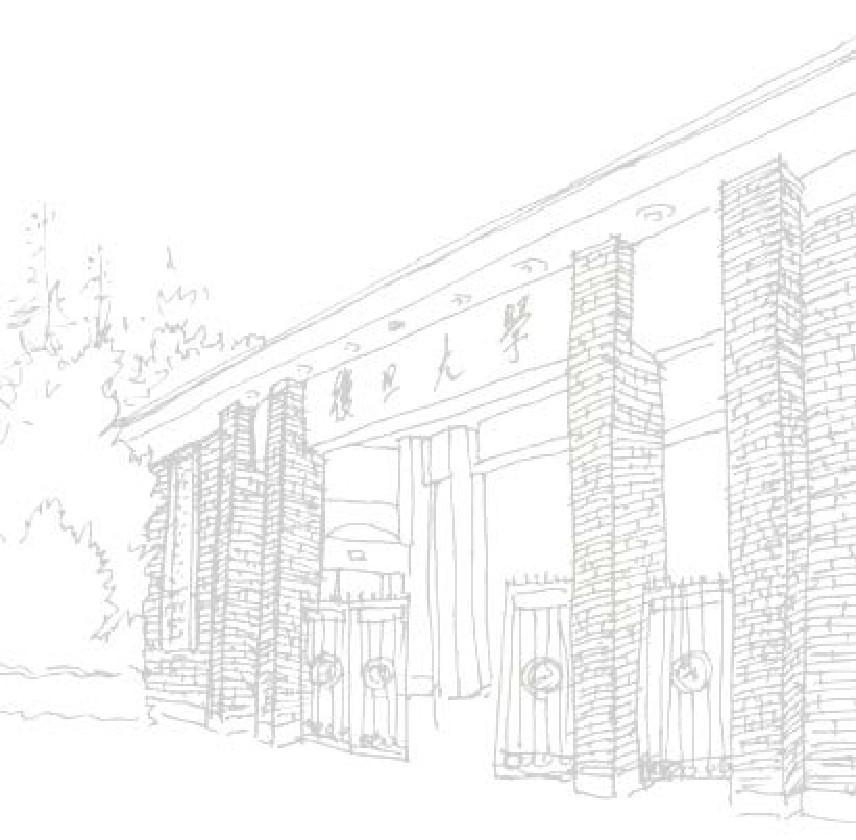
\includegraphics[scale=0.2]{maingate2}}
\begin{document}

\begin{frame}
\titlepage
\end{frame}

\begin{frame}{Overview}
\tableofcontents
\end{frame}
%------------------------------------------------
\section{Introduction}
\begin{frame}{Research Territory}{Imperfect Competition for International Trade}
	\begin{itemize}
		\item Models of imperfect competition for international trade
		\item Applied work is limited \\
		Dixit (1988) and Krishna et al.(1989):Calibration \\
		Feenstra (1984, 1985, 1988), Levinsohn (1988), and Feenstra and Levinsohn (1989): on automobile market
		\item Trade policy on welfare \\
		Need an econometric model for applied work
	\end{itemize}
\end{frame}
%------------------------------------------------
\begin{frame}{Research Niche}{Imperfect Competition on Automobile Industry}
\begin{itemize}
	\item Number of competing firms is small enough to justify the assumption of oligopoly
	\item Products are highly differentiated
	\item A major target of trade policy
	\begin{block}{Trade Policy}
		\begin{itemize}
			\item (1980s) Imports tariff of cars is 2.9 percent
			\item (1980s) Imports tariff of compact trucks is 25 percent
			\item (1981.5) "Voluntary Export Restraint" (VER) for Japanese auto sales
		\end{itemize}
	\end{block}
\end{itemize}
\end{frame}
%------------------------------------------------
\begin{frame}{Previous Research}
	\begin{block}{Use Disaggregate Consumer Data}
	\textbf{Advantages}
		\begin{itemize}
	\item Composed of logit-based models that estimate automobile demand at the individual level
	\item Allow for a high degree of product differentiation and account for consumer heterogeneity
	\item Circumvent the problem of price endogeneity
		\end{itemize}
	\textbf{Disdvantages}
		\begin{itemize}
	\item Neglect supply side and market equilibrium consideration
	\item Inadequate in a forecasting context, as prices are determined by market forces
	\item Limits the use of such approaches for policy formulation
		\end{itemize}
	\end{block}
\end{frame}
%------------------------------------------------
\begin{frame}{Previous Research}
	\begin{block}{Use Aggregate Consumer Data}
	\textbf{Disdvantages}
	\begin{itemize}
	\item Endogeneity of prices
	\item The existence of a well defined reduced form often requires strong assumptions about the functional form of the demand system
	\end{itemize}
	\end{block}
\begin{itemize}
	\item Ignore the existence of an outside good \\
	Impossible to derive the aggregate demand curve
\end{itemize}
\end{frame}
%------------------------------------------------
\begin{frame}{Present Research}
	\begin{itemize}
		\item Model \\
		Combining a disaggregate model of automobile demand with an aggregate oligopoly model
		\item Discrete choice model of demand \\
		- Nested logit model \\
		- Micro data from the Consumer Expenditure Surve \\
		- Combined with population weight to determine aggregate demand
		\item Supply side \\
		- An oligopoly with differentiated products \\
		- Nash Equilibrium with prices as strategic variables
	\end{itemize}
\end{frame}
%------------------------------------------------
\begin{frame}{Present Research}{Topic of Interest}
\begin{itemize}
	\item Quota Restrictions \\~\\
	\item Exchange Rate Pass-through \\
	- Quantify the effects of the VER on market shares, automobile prices, and quality upgrading \\
	- Compare quotas to an equivalent tariff, find different effect on prices  \\~\\
	\item Explanation for insensitivity of import prices to exchange rate movements \\
	- Estimate the effects of exchange rates on import prices \\
	- Assess the significance of trade restrictions, quality upgrading, and exchange rate pass-through on prices 
\end{itemize}
\end{frame}
%------------------------------------------------
\section{Automobile Market Model}
\begin{frame}{Automobile Choice Model}
Consumers are assumed to maximize an indirect utility function of the form
$$U_{j}^{h}=\bar{V}_{j}^{h}+\varepsilon_{j}^{h}$$
where $j$ and $h$ stand for vehicle and household \\~\\
$\bar{V}_{j}^{h}$ the utility function from the vehicles and the consumer's characteristics \\~\\
$\varepsilon_{j}^{h}$ captures the effects of unmeasured variables, personal idiosyncrasies, maximization error \\~\\
Partition the whole set of vehicles into k disjoint subsets according to the criteria of newness (n), market segment (c), and origin (o), so that each vehicle make (m) is indexed by (n, c, o, m)
$$U_{b, n, c, o, m}^{h}=\bar{V}_{b, n, c, o, m}^{h}+\varepsilon_{b, n, c, o, m}^{h}$$
where the subscript $b$ stands for buy
\end{frame}
%------------------------------------------------
\begin{frame}{Automobile Choice Model}
Assume that $\bar{V}$ is a linear function of consumer and vehicle characteristics \\~\\
$U_{b, n, c, o, m}^{h}= \alpha^{\prime} B_{b}^{h}+\beta^{\prime} N_{b, n}^{h}+\gamma^{\prime} C_{b, n, c}^{h}+\delta^{\prime} O_{b, n, c, o}^{h}+\zeta^{\prime} M_{b, n, c, o, m}^{h}+\varepsilon_{b, n, c, o, m}^{h}$ \\~\\
\begin{itemize}
	\item The decision to purchase
	\item Utility derived from owning a new as opposed to used car
	\item Owning a car of a particular market segment, origin, and make, respectively \\
	- A car's make is the brand of the vehicle, while the model refers to the name of a car product and sometimes a range of products
\end{itemize}
Assume the error term follows the generalized EVD \\~\\
The joint probability of choosing a new vehicle type
$$P_{b, n, c, o, m}^{h}=P_{b}^{h} * P_{n / b}^{h} * P_{c / n, b}^{h} * P_{o / c, n, b}^{h} * P_{m / o, c, n, b}^{h}$$
\end{frame}
%------------------------------------------------
\begin{frame}{Automobile Choice Model}
\begin{itemize}
	\item Nested Logit:McFadden (1978)
\end{itemize}
\begin{figure}[h]
	\centering
	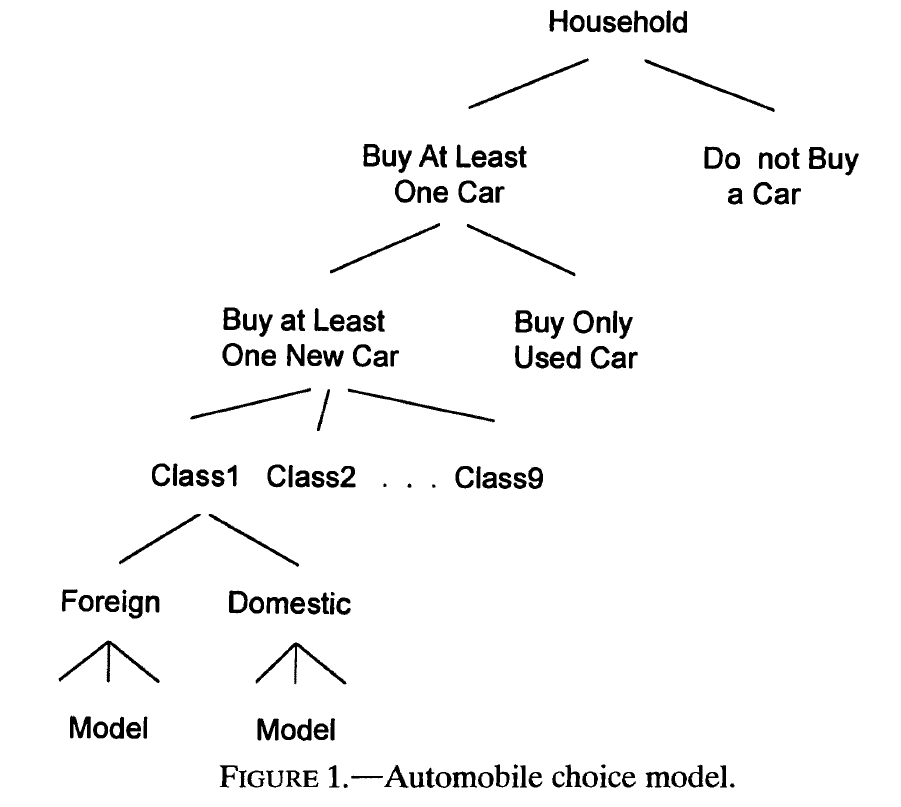
\includegraphics[width=8cm]{Figure1.png}
\end{figure}
\end{frame}
%------------------------------------------------
\begin{frame}{Automobile Choice Model}
\begin{itemize}
	\item Nested Logit:McFadden (1978) \\
	$$\zeta^{\prime} M_{b, n, c, o, m}^{h}=\zeta_{1}^{\prime} M 1_{b, n, c, o, m}^{h}+\zeta_{2}\left(I N C^{h}-P R I C E_{b, n, c, o, m}\right)$$
	The vector $M_{b, n, c, o, m}^{h}$ includes all relevant characteristics other than price and income, $INC$ stands for income of household $h$, and $\zeta_{2}$ is the price parameter to be estimated
\end{itemize}
\end{frame}
%------------------------------------------------
\begin{frame}{Aggregation}
\begin{itemize}
	\item Aggregate demand is defined as the sum of individual household demands
	\item Consumer Expenditure Survey provides weights for each household,reflecting the representativeness of that household in the United States population
	\item Aggregate Demand
	$$D_{b, n, c, o, m}=\sum_{h} P_{b, n, c, o, m}^{h} w^{h}+\sum_{h} \eta_{b, n, c, o, m}^{h} w^{h}$$
	$P_{b, n, c, o, m}^{h}$ is selection probability, $w^{h}$ is the individual household weight, $\eta_{b, n, c, o, m}^{h}$ is a mean zero, stochastic component that is not observed by either the econometrician or the firm
	\item Expected Demand
	$$ED_{b, n, c, o, m}=\sum_{h} P_{b, n, c, o, m}^{h} w^{h}$$
\end{itemize}
\end{frame}
%------------------------------------------------
\begin{frame}{Aggregation}{Supply Side and Market Equilibrium}
The firms participating in the market are of three types: domestic, foreign non-Japanese, and Japanese producers facing the VER
$$\max _{p_{i t}^{w}} E_{t} \Pi_{t}^{f}=E_{t}\left\{\sum_{i=1}^{n_{f t}}\left(p_{i t}^{w}-c_{i t}\right) q_{i t}-F_{f t}\left(X_{f t}\right)\right\}$$
At equilibrium:
$$E_{t} q_{i t}=E_{t} D_{i t}=E_{t}\left\{\sum_{h} P_{i t}^{h} w^{h}+\sum_{h} \eta_{i t}^{h} w^{h}\right\}=\sum_{h} P_{i t}^{h} w^{h}$$
For foreign producers:
$$\max _{p_{t t}^{w}, \lambda_{f t}} E_{t} L_{t}^{f}=E_{t}\left\{\sum_{i=1}^{n_{f t}}\left(e_{t} p_{i t}^{w}-c_{i t}\right) q_{i t}-F_{f t}\left(X_{f t}\right)+\lambda_{f t}\left(D_{f t}-\sum_{j^{\prime} \in V_{f}} q_{j^{\prime} t}\right)\right\}$$
\end{frame}
%------------------------------------------------
\begin{frame}{Aggregation}{Subject to Quota}
	(a) Domestic Firm: \\
	$E_{t} D_{i t}+\sum_{j=1}^{n_{f t}}\left(p_{j t}^{w}-c_{j t}\right) \frac{\partial E_{t} D_{j t}}{\partial p_{i t}^{w}}=0 \quad\left(i=1, \ldots, n_{f}\right)$ \\~\\
	(b) Foreign Firm: \\
	$e_{t} E_{t} D_{i t}+\sum_{j=1}^{n_{f t}}\left(e_{t} p_{j t}^{w}-c_{j t}\right) \frac{\partial E_{t} D_{j t}}{\partial p_{i t}^{w}}=0 \quad\left(i=1, \ldots, n_{f}\right)$ \\~\\
	(c) "Subject to Quotas" Foreign Firm: \\
	$e_{t} E_{t} D_{i t}+\sum_{j=1}^{n_{f t}}\left(e_{t} p_{j t}^{w}-c_{j t}\right) \frac{\partial E_{t} D_{j t}}{\partial p_{i t}^{w}}-\lambda_{f t} \sum_{j^{\prime} \in V_{f}} \frac{\partial E_{t} D_{j^{\prime} t}}{\partial p_{i t}^{w}}=0$ \\~\\
	$\sum_{j^{\prime} \in V_{f}} E_{t} D_{j^{\prime} t} \leqslant D_{f t}, \quad \lambda_{f t} \geqslant 0$
\end{frame}
%------------------------------------------------
\section{Data}
\begin{frame}{Data Description}
\begin{itemize}
	\item Consumer Expenditure Survey \\~\\
	Since 1984 the CES also contains detailed information on the automobile holdings of the interviewed households, including the \textbf{make/model and purchase price of each car} and a large set of vehicle characteristics \\~\\
	A comparison with Census data shows that the sample is representative of the U.S. population
\end{itemize}
\end{frame}
%------------------------------------------------
\begin{frame}{Data Description}
\begin{itemize}
	\item Potential Problem1 \\
	- Only nine percent of the sample households purchase a new vehicle each year, which seems to underestimate the total sales of new vehicles in the United States. \\
	- It is consistent with other publications of the Bureau of Labor Statistics and the U.S. Department of Commerce \\
	- One explanation for this divergence is the existence of fleet sales
	\item Potential Problem2 \\
	- New car models in the sample is relatively small \\
	- Limit the ability to introduce model fixed effects
	\item The CES was supplemented by information on approximately 200 models per year for the period 1983-87
\end{itemize}
\end{frame}
%------------------------------------------------
\section{Identification Assumptions}
\begin{frame}[shrink]
	\transfade %fade in and fade out
	\tableofcontents[sectionstyle=show/shaded,subsectionstyle=show/shaded/hide]
	\addtocounter{framenumber}{-1}
\end{frame}
%------------------------------------------------
\begin{frame}{Identification Assumptions}
	The main identification assumption is that the variables on the right-hand side of the demand system are uncorrelated with the individual error term in the demand equation.
	
	Among the variables included in the demand equation, there are two sets for which the above assumption may seem suspect:
	\begin{itemize}
		\item existing stock of cars;
		\item prices.
	\end{itemize}
\end{frame}
%------------------------------------------------
\begin{frame}{Identification Assumptions}{The Existing Stock of Cars}
	\begin{itemize}
		\item This issue is identical to the ones associated with the use of lagged dependent variables; if the error term of the demand equation is serially correlated, the obtained parameter estimates are inconsistent.
		\item However, dealing with serial correlation in the nested logit model is difficult. Eliminating these variables from the demand estimation would lead to implausible purchasing patterns, as the decision to buy clearly depends on the current stock.
		\item Therefore, I maintain the assumption that the error terms in the demand specification are not serially correlated.
	\end{itemize}
\end{frame}
%------------------------------------------------
\begin{frame}{Identification Assumptions}{Prices}
	Similarly, I assume that prices are not correlated with the consumer specific error term of the demand equation. This assumption is justified on the basis of two considerations:
	\begin{itemize}
		\item Use of micro data;
		\item Expected profit maximization.
	\end{itemize}
\end{frame}
%------------------------------------------------
\begin{frame}{Identification Assumptions}{Prices}
	Use of micro data: In principle, an aggregate component in the error term can arise from two sources:
	\begin{itemize}
		\item The first source is a macroeconomic shock, such as a recession. Such a shock manifests itself in household characteristics that are observed, such as income, employment status, assets, etc. By controlling for these variables in the demand estimation I remove the aggregate component from the error terms.
	\end{itemize}
\end{frame}
%------------------------------------------------
\begin{frame}{Identification Assumptions}{Prices}
	\begin{itemize}
		\item A second aggregate component in the error term is unobserved product characteristics that are perceived in the same way by all consumers. Micro data allow one to estimate this aggregate component as a fixed effect. In this presence, the utility function becomes
		\begin{equation}
			U_j^h = \bar{V}_j^h + \xi_j + \varepsilon_j^h.
		\end{equation}
		\item In the current data set, however, new automobile models are sometimes associated with only one observation in the sample so that model specific effects cannot be estimated.
		\item To accommodate this unfortunate feature, I decompose the product specific unobserved attributes $\xi_j$ into market segment component $\xi_j^c$, origin component $\xi_j^o$, and brand compotent $\xi_j^{br}$:
		\begin{equation}
			\xi_j = \xi_j^c + \xi_j^o + \xi_j^{br}.
		\end{equation}
	\end{itemize}
\end{frame}
%------------------------------------------------
\begin{frame}{Identification Assumptions}{Prices}
	\begin{itemize}
		\item The second argument supporting the exogeneity of prices comes from the assumption that producers maximize expected profits. This assumption implies that under fairly general conditions prices are uncorrelated with the demand error.
		\item To clarify, let us without loss of generality focus on the maximization problem of a domestic producer.
		\begin{equation}
			\max_{p^w_{it}} E_t\left\{\sum_{i=1}^{n_{ft}}(p_{it}^w-c_{it})\left(\sum_h p_{it}^hw^h+\sum_h\varepsilon_{it}^hw^h\right) \right\}.
		\end{equation}
	\end{itemize}
\end{frame}
%------------------------------------------------
\begin{frame}{Identification Assumptions}{Prices}
	\begin{itemize}
		\item Firms observe the actual marginal cost $c_{it}$ while the econometrician only observes the deterministic component $\bar{c}_{it}$. Thus from the econometrician's perspective the supplier's problem is
		\begin{equation}
			\max_{p^w_{it}} E_t\left\{\sum_{i=1}^{n_{ft}}(p_{it}^w-\bar{c}_{it}-u_{it})\left(\sum_h p_{it}^hw^h+\sum_h\varepsilon_{it}^hw^h\right) \right\}.
		\end{equation}
		\item Assuming that the error terms of the cost and demand equations, $u_{it}$ and $\varepsilon_{it}^h$ are independent, the demand error drops out of the maximization condition so that it does not affect the determination of prices.
		\begin{equation}
			\Rightarrow\quad \max_{p^w_{it}} E_t\left\{\sum_{i=1}^{n_{ft}}(p_{it}^w-\bar{c}_{it}-u_{it})\sum_h p_{it}^hw^h \right\}.
		\end{equation}
	\end{itemize}
\end{frame}
%------------------------------------------------

%------------------------------------------------
\section{Empirical Results and Interpretation}
\begin{frame}[shrink]
	\transfade %fade in and fade out
	\tableofcontents[sectionstyle=show/shaded,subsectionstyle=show/shaded/hide]
	\addtocounter{framenumber}{-1}
\end{frame}
%------------------------------------------------
\begin{frame}{Empirical Results and Interpretation}
	This section summarizes the results from the estimation of the demand and supply systems.
	\begin{itemize}
		\item First, I present the results from estimating the automobile choice model and testing alternative specifications.
		\item Next, I analyze the implications of the estimated parameters for aggregate market shares and price elasticities of demand.
		\item Finally I report the supply side results, with emphasis on the marginal costs, markups, and cost parameters implied by the model.
	\end{itemize}
\end{frame}
%------------------------------------------------
\begin{frame}{Estimation Results of the Automobile Choice Model}{Model Choice}
	\begin{columns}
		\column{0.33\textwidth}
		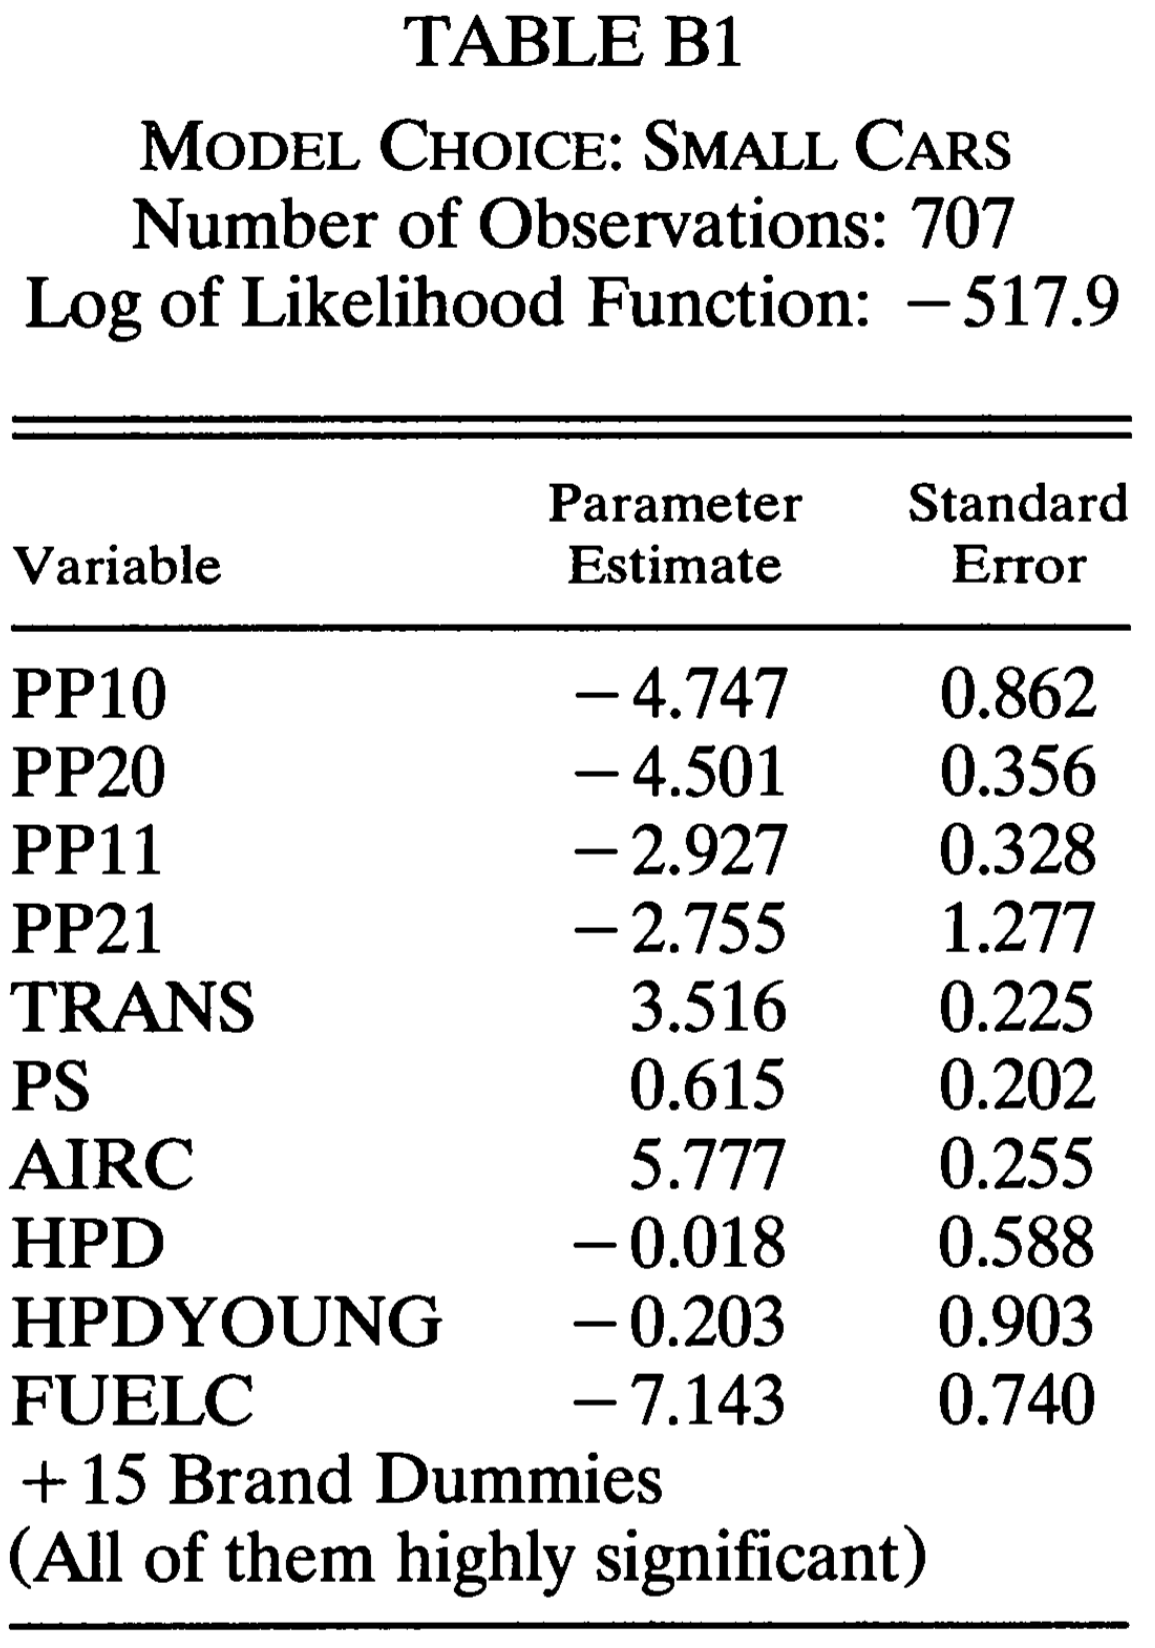
\includegraphics[width=3.5cm]{table_b1.png}
		\column{0.33\textwidth}
		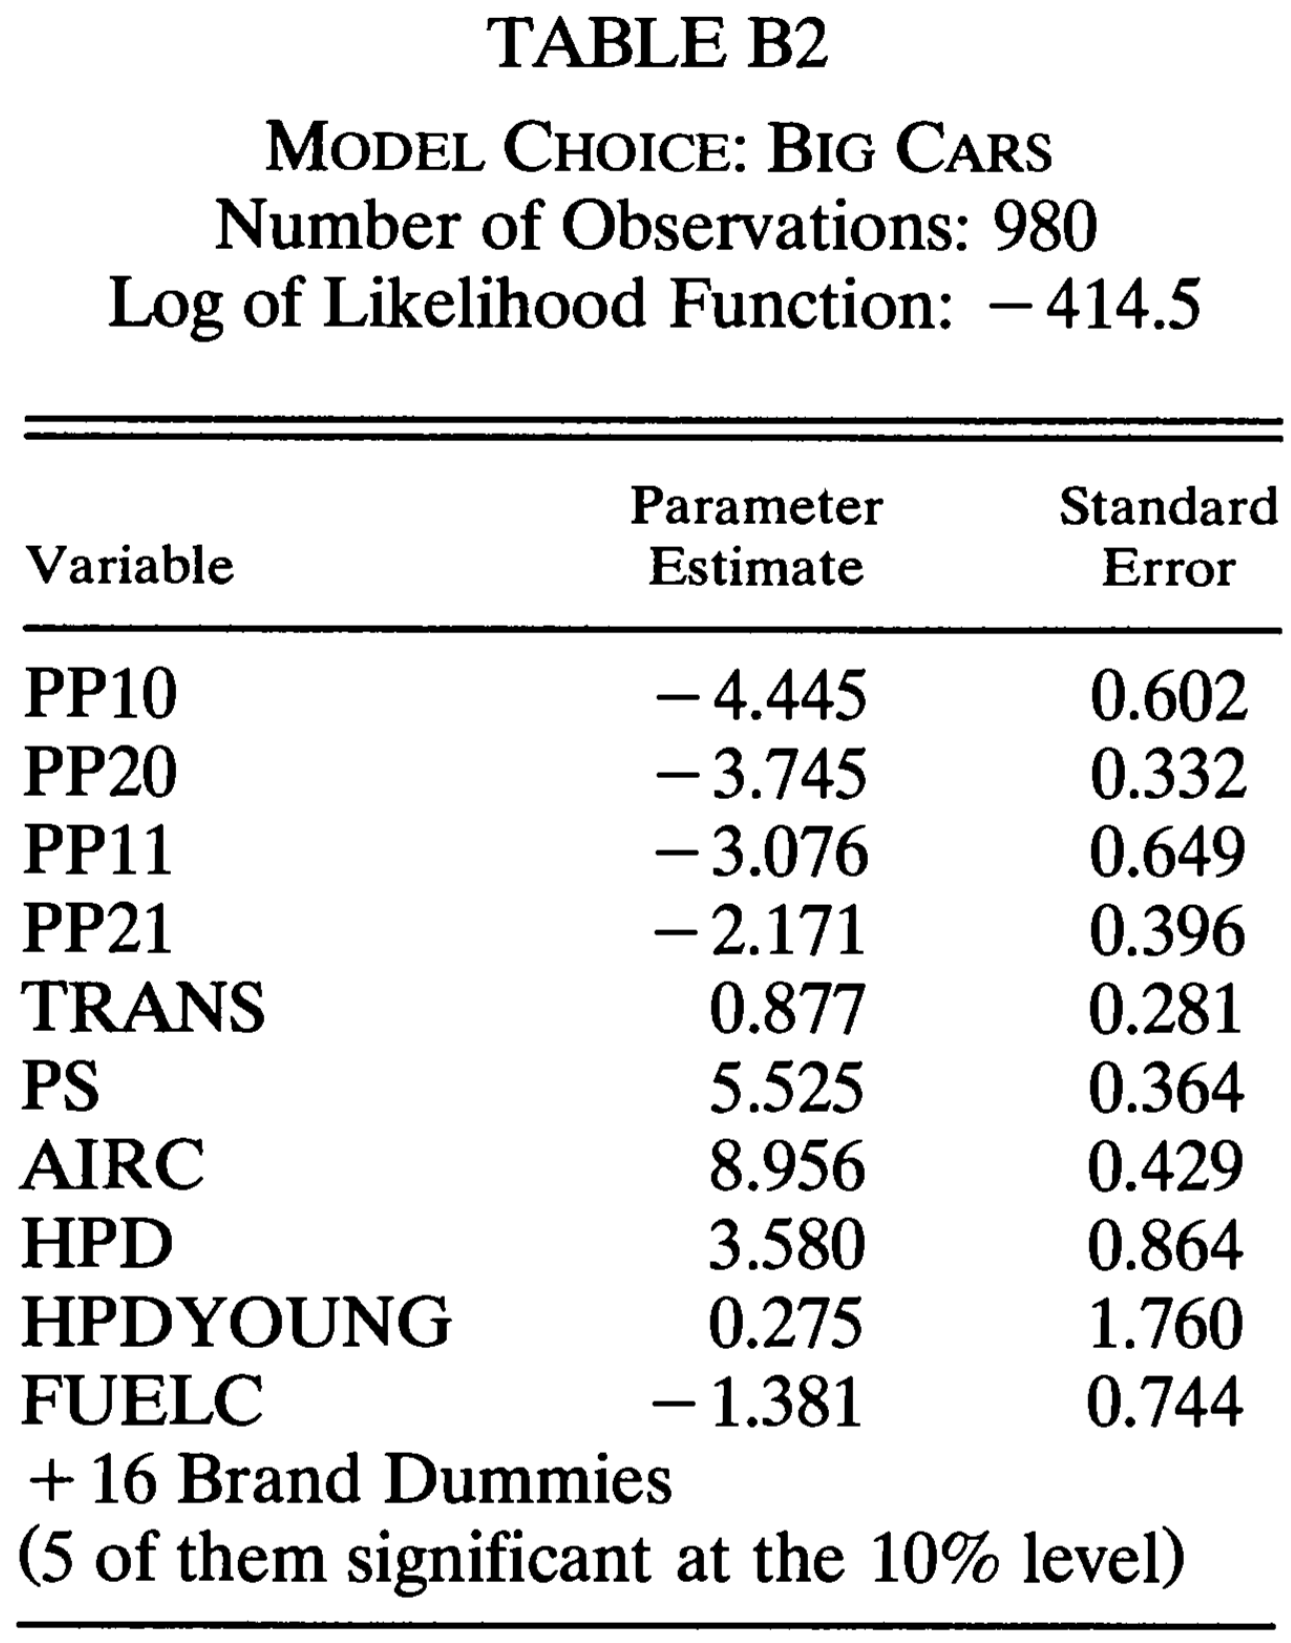
\includegraphics[width=3.7cm]{table_b2.png}
		\column{0.33\textwidth}
		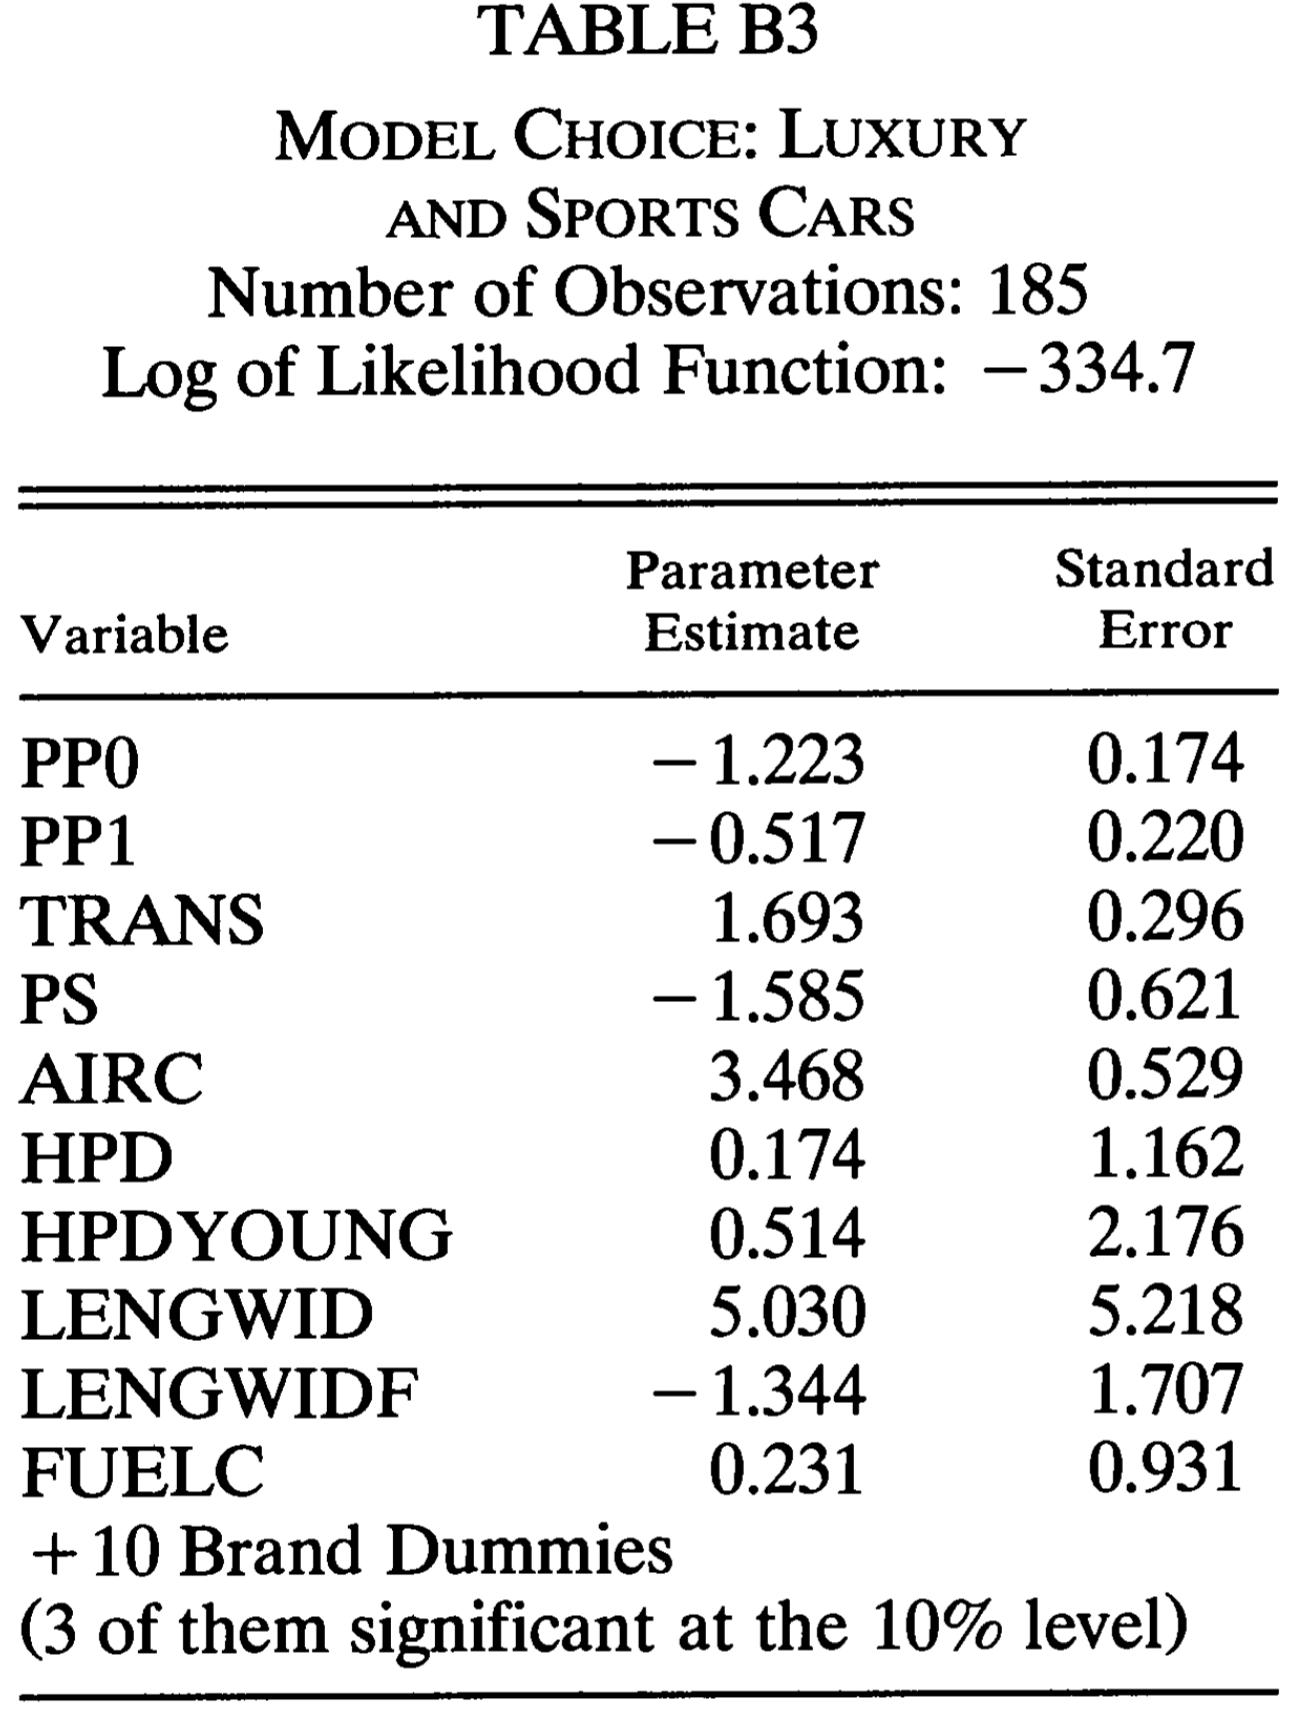
\includegraphics[width=3.5cm]{table_b3.png}
	\end{columns}
\end{frame}
%------------------------------------------------
\begin{frame}{Estimation Results of the Automobile Choice Model}{Foreign vs. Domestic}
	\begin{figure}[h]
		\centering
		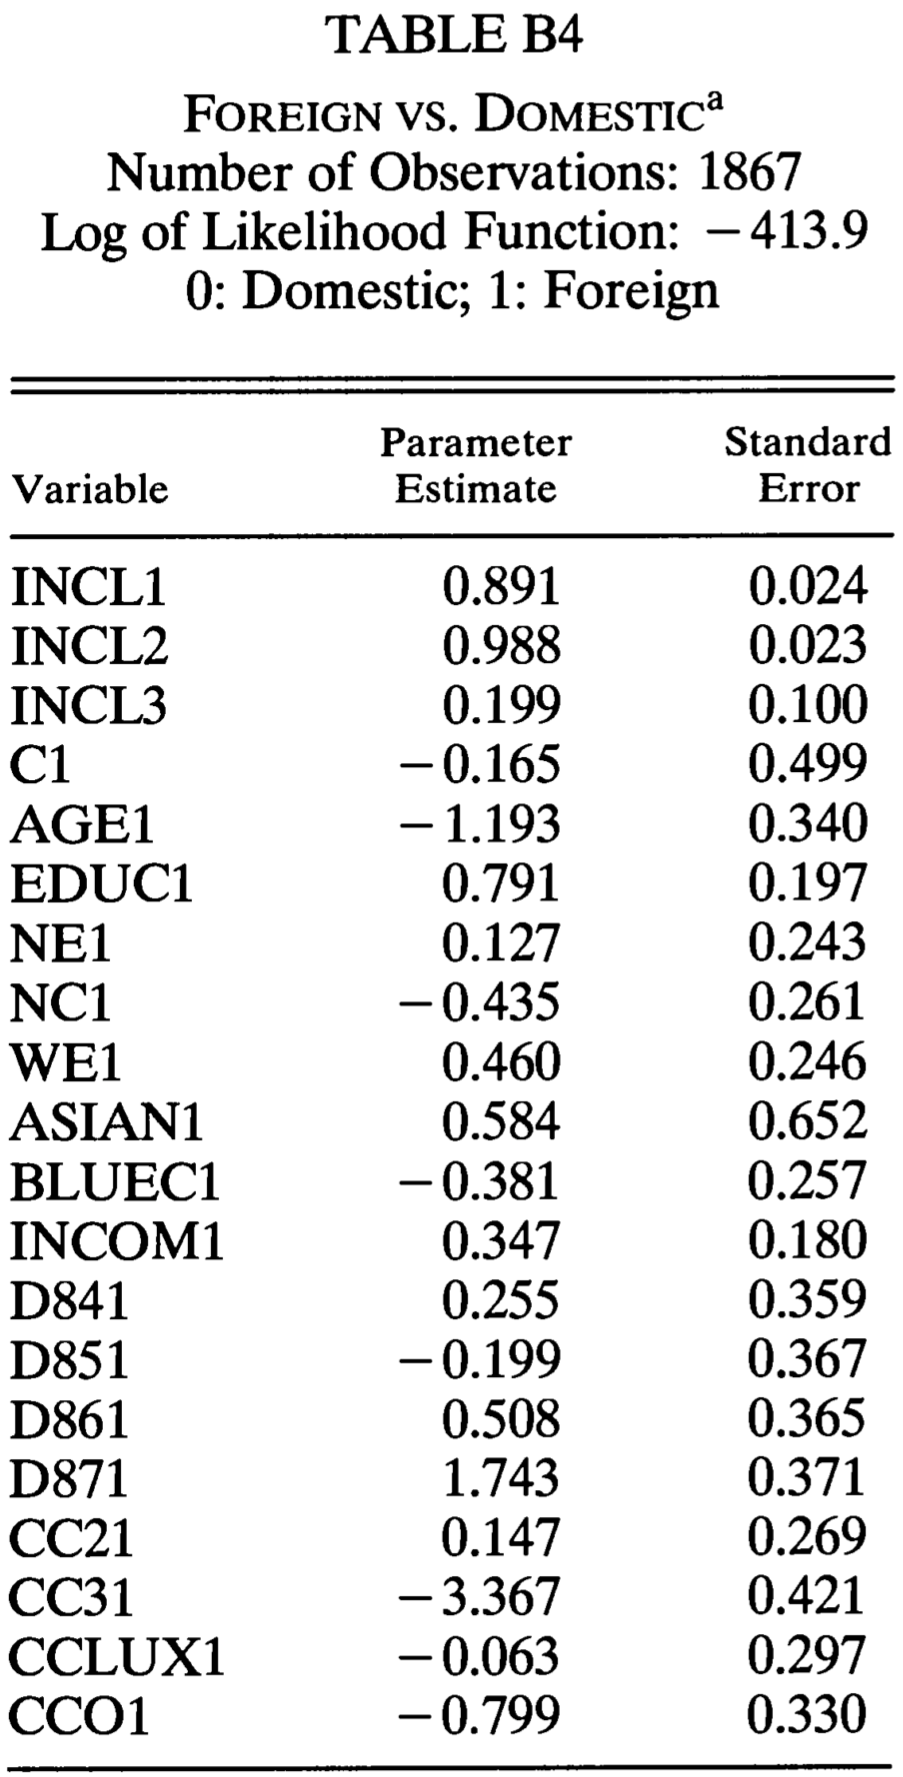
\includegraphics[scale=0.32]{table_b4.png}
	\end{figure}
\end{frame}
%------------------------------------------------
\begin{frame}{Estimation Results of the Automobile Choice Model}{Class Choice}
	\begin{columns}
		\column{0.5\textwidth}
		\begin{figure}[h]
			\centering
			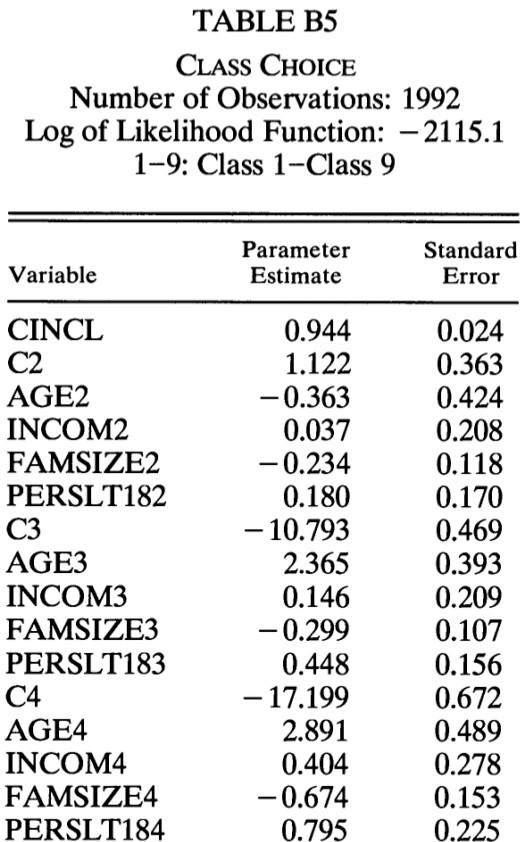
\includegraphics[width=4.6cm]{table_b51.png}
		\end{figure}
		\column{0.5\textwidth}
		\begin{figure}[h]
			\centering
			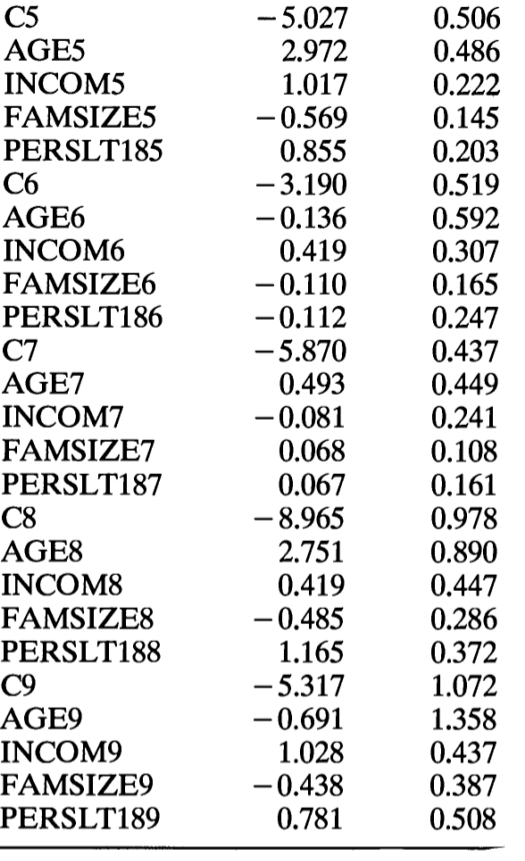
\includegraphics[width=4.6cm]{table_b52.png}
		\end{figure}
	\end{columns}
\end{frame}
%------------------------------------------------
\begin{frame}{Estimation Results of the Automobile Choice Model}{Used vs. New and Buy vs. Not Buy}
	\begin{columns}
		\column{0.5\textwidth}
		\begin{figure}[h]
			\centering
			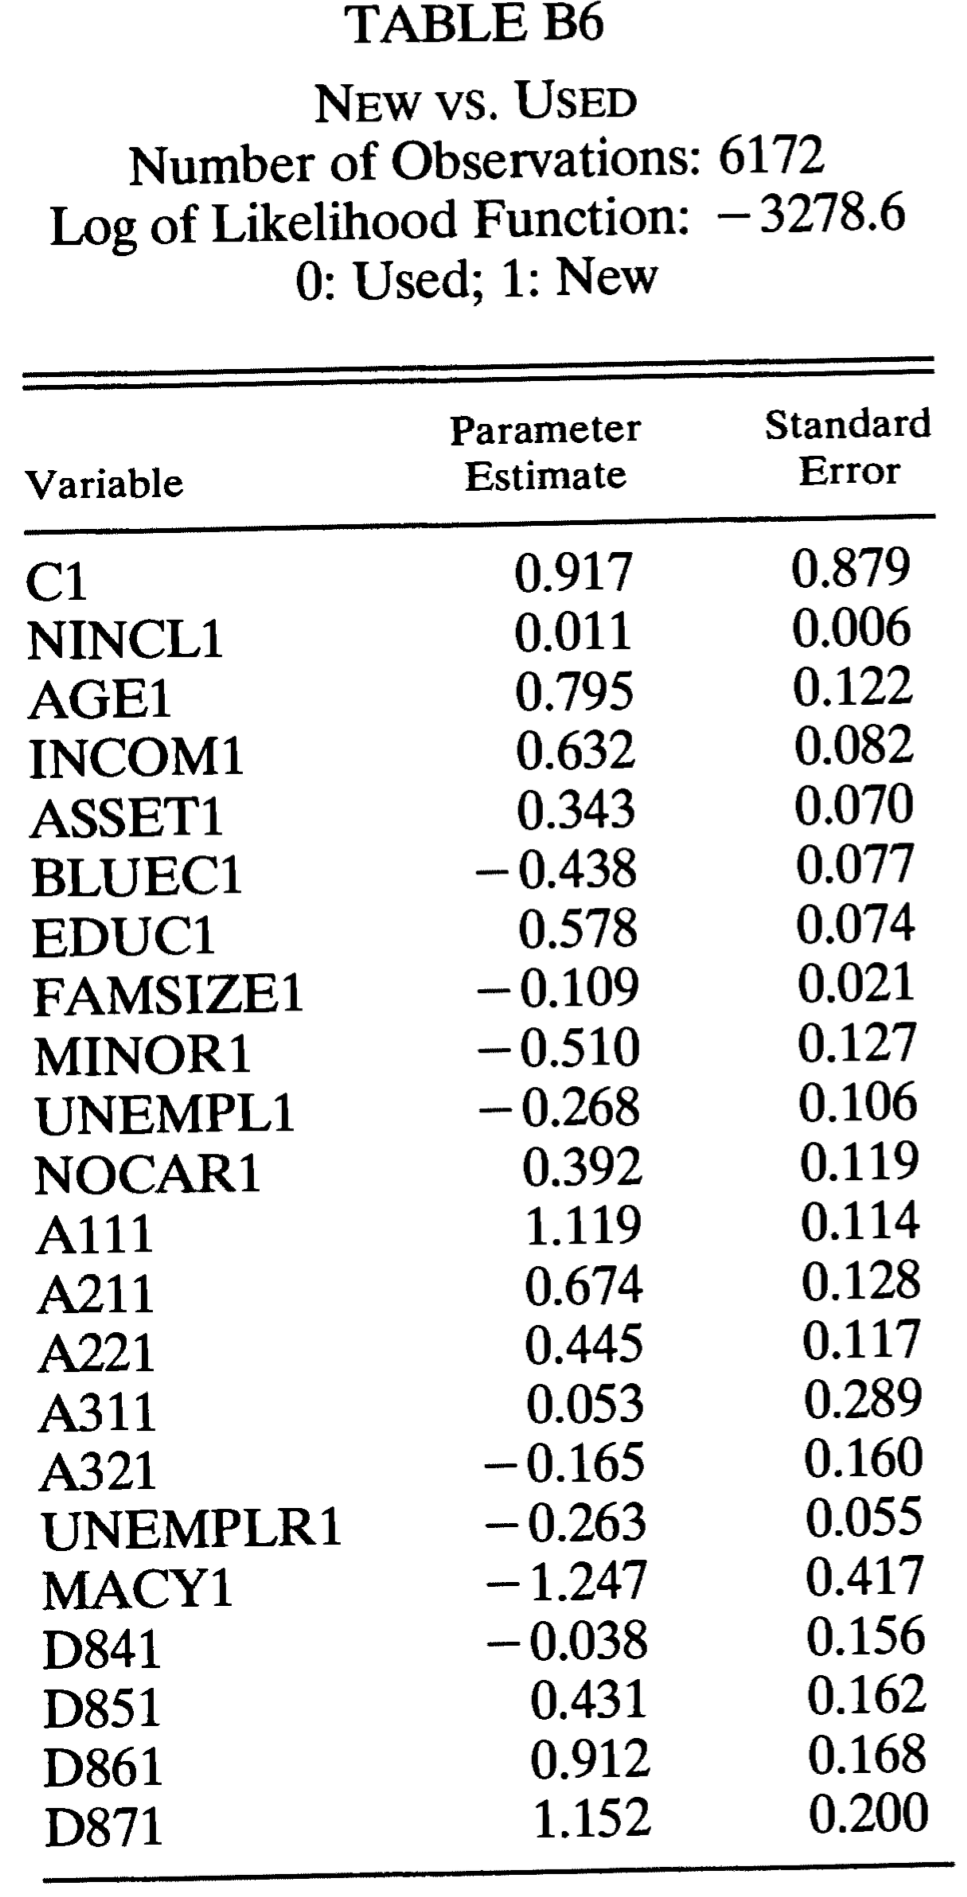
\includegraphics[width=3.8cm]{table_b6.png}
		\end{figure}
		\column{0.5\textwidth}
		\begin{figure}[h]
			\centering
			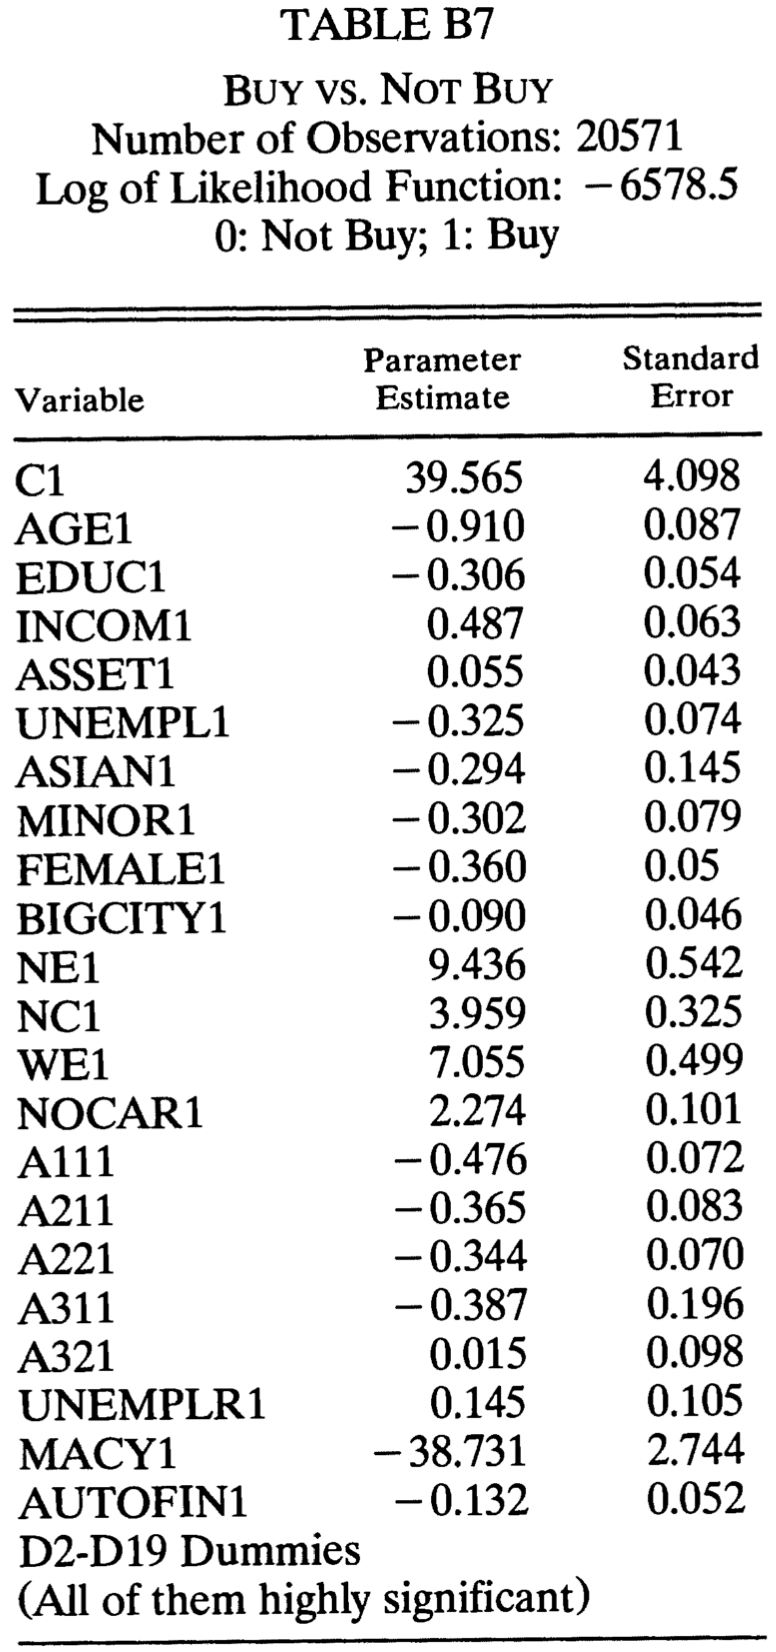
\includegraphics[width=3.5cm]{table_b7.png}
		\end{figure}
	\end{columns}
\end{frame}
%------------------------------------------------
\begin{frame}{Specification Testing}{Alternative Specifications}
	\begin{equation}
		T=\left(\hat{\beta}_r-\hat{\beta}_u\right)'\left(\hat{V}_r-\hat{V}_u\right)^{-1}\left(\hat{\beta}_r-\hat{\beta}_u\right)
	\end{equation}
	\begin{figure}[h]
		\centering
		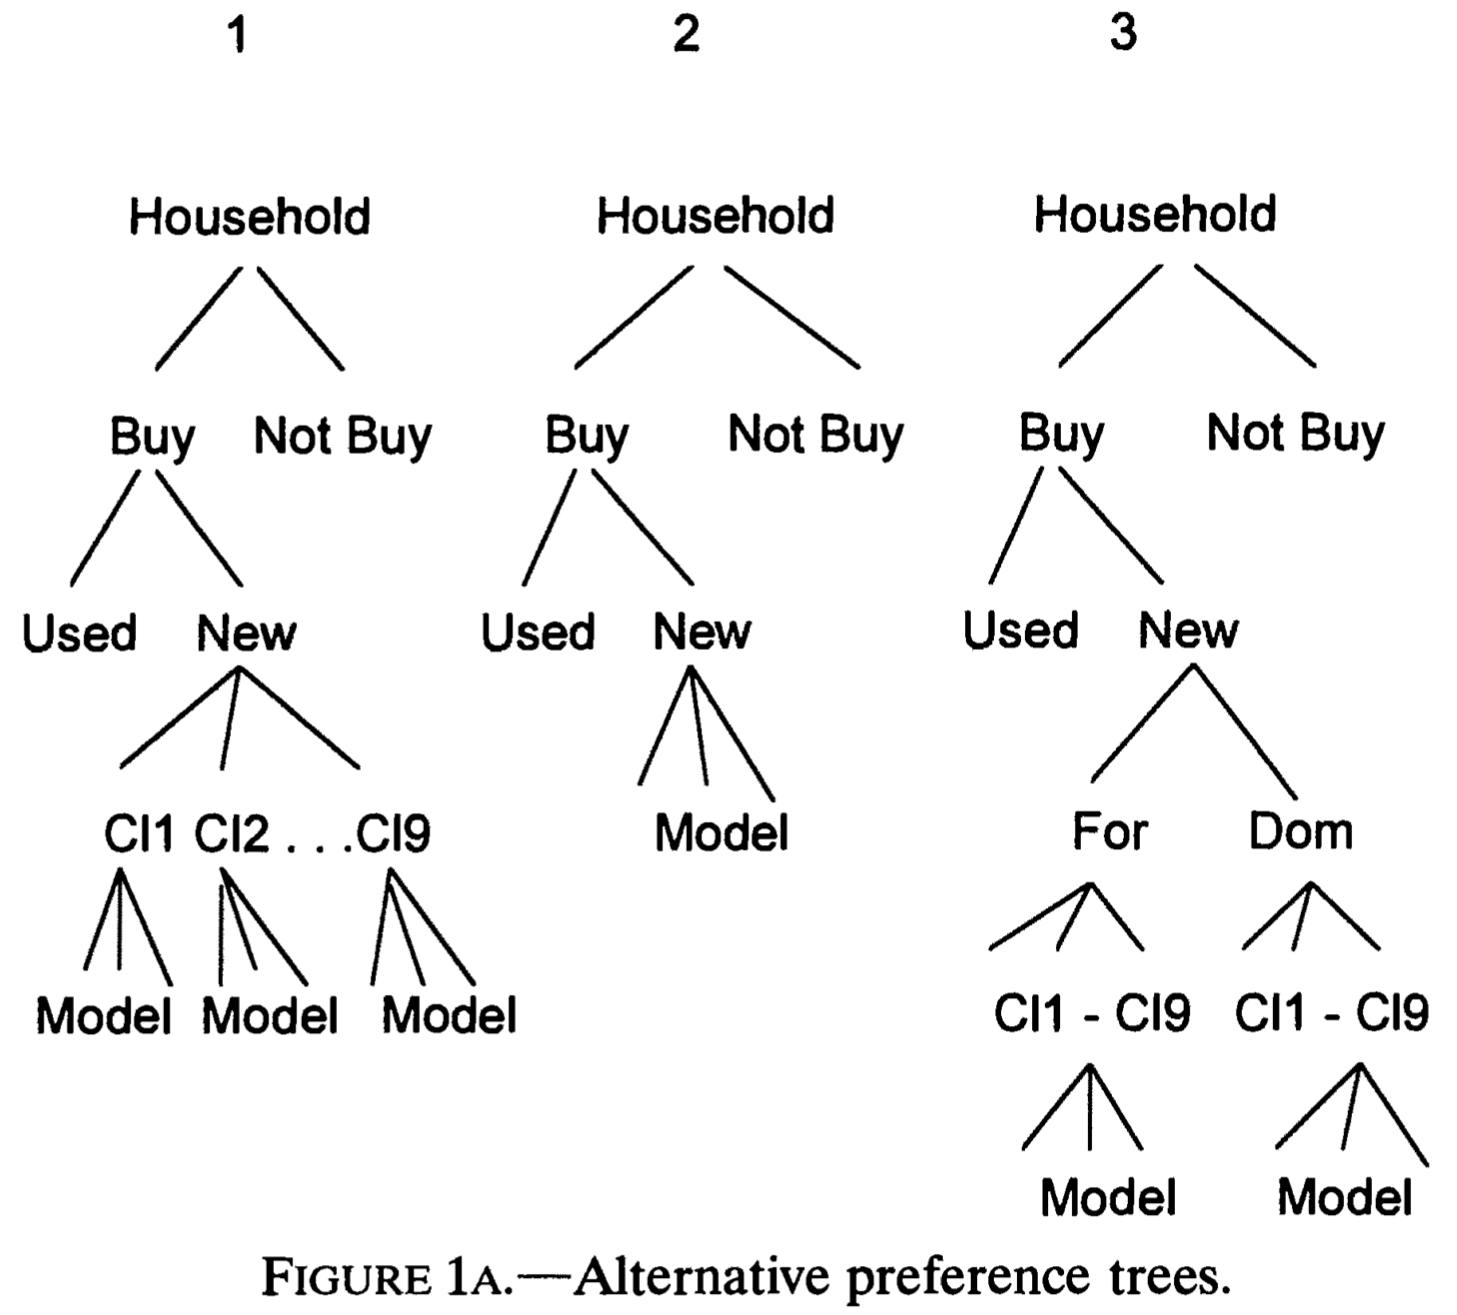
\includegraphics[scale=0.35]{figure_1a.png}
	\end{figure}
\end{frame}
%------------------------------------------------
\begin{frame}{Specification Testing}{Alternative Specifications}
	\begin{figure}[h]
		\centering
		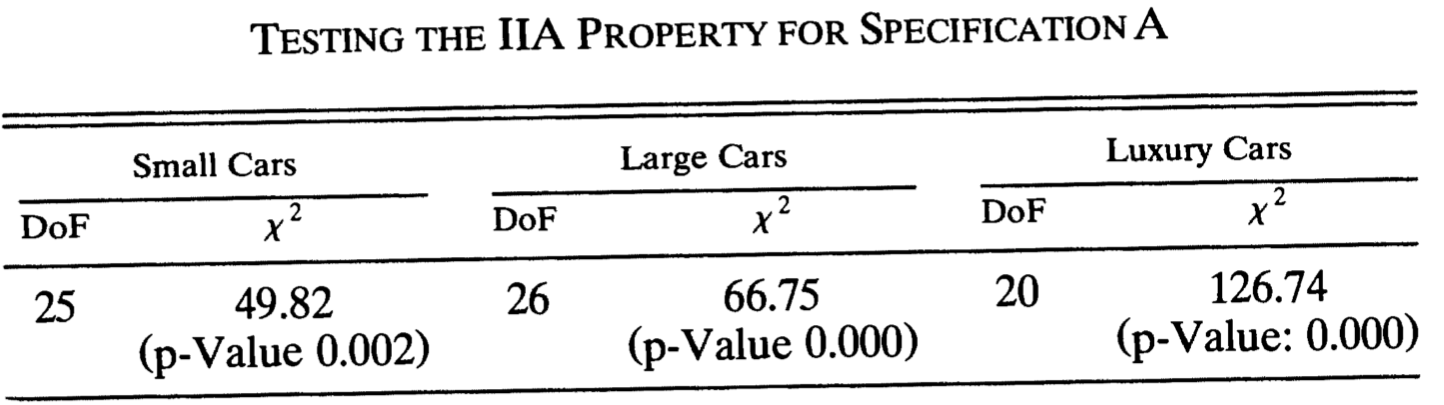
\includegraphics[scale=0.45]{table_c1(2).png}
		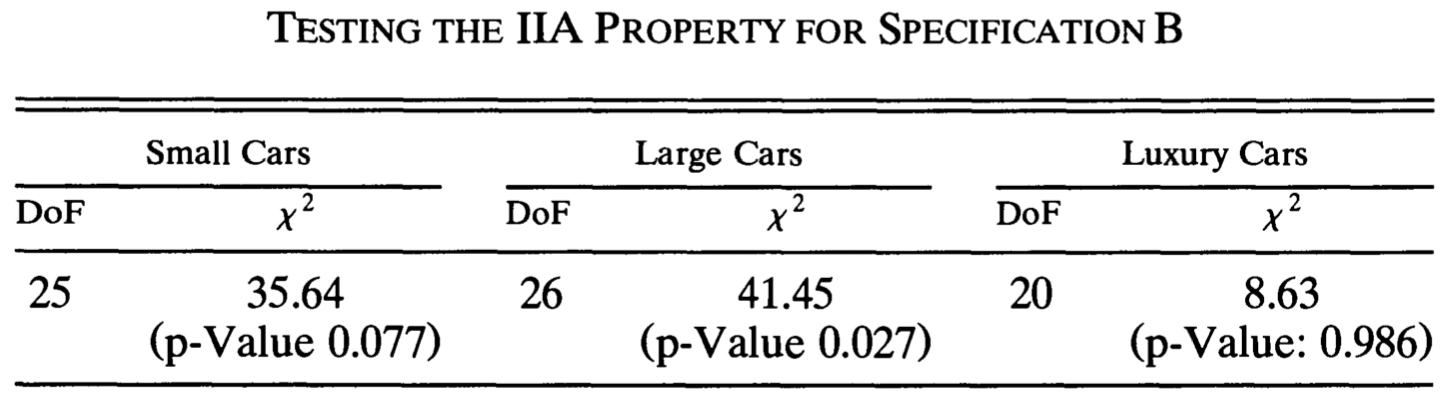
\includegraphics[scale=0.45]{table_c2(2).png}
		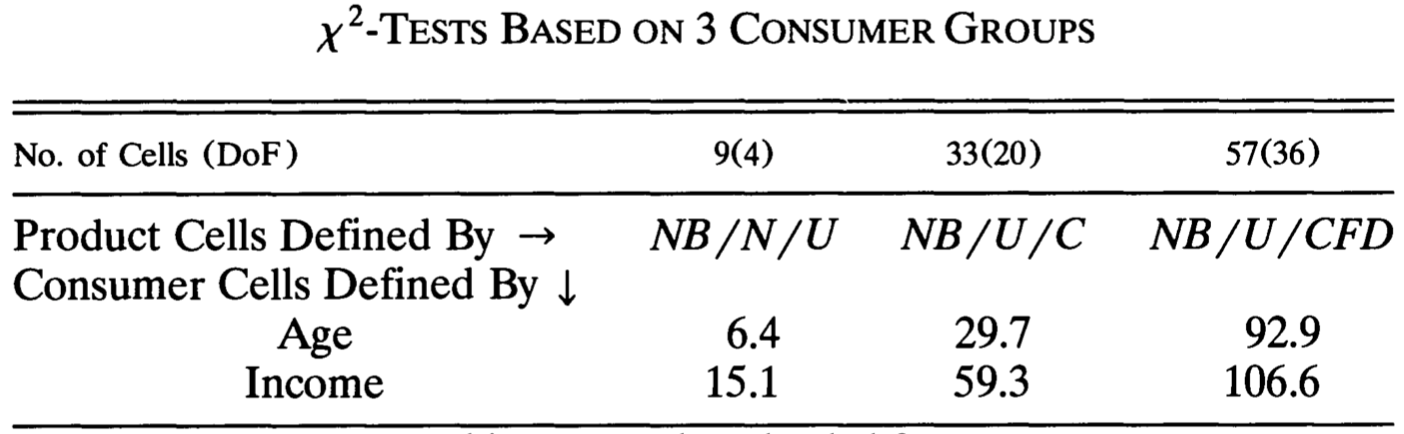
\includegraphics[scale=0.45]{table_c3(2).png}
	\end{figure}
\end{frame}
%------------------------------------------------
\begin{frame}{Specification Testing}{Alternative Specifications}
	\begin{itemize}
		\item In summary, the model estimated in the previous section is the only one among the alternatives considered here that is consistent with random utility maximization and does not violate the IIA assumption at each node of the tree.
	\end{itemize}
\end{frame}
%------------------------------------------------
\begin{frame}{Specification Testing}{The Fit of the Model}
	Aggregate Market Shares: The difference between actual and expected ones can be split in two components:
	\begin{itemize}
		\item Discrepancy between the CES and the actual market shares: sampling error problem.
		\item Discrepancy between expected and actual aggregate market shares: difference between estimated and CES shares.
		\begin{itemize}
			\item The estimation procedure predicts the CES market shares at the higher nodes of the tree exactly. The specification includes choice specific dummies and time effects, so that at the aggregate the model fits the data exactly.
			\item The last stage includes brand but not model specific dummies; the predicted aggregate market shares for specific vehicle makes deviate from the actual CES shares. This deviation turns out quite small, suggesting that potential simultaneity bias due to the omission of choice specific dummies at the lower level is not important.
		\end{itemize}
	\end{itemize}
\end{frame}
%------------------------------------------------
\begin{frame}{Specification Testing}{The Fit of the Model}
	$\chi^2$ Tests: A better idea about the fit of the model can be obtained by performing $\chi^2$ tests at a more disaggregate level based on finer consumer and vehicle classifications.

	Main findings:
	\begin{itemize}
		\item The results are sensitive to both the number of cells and the way the cells are defined; increasing the number of cells tends to increase the probability of rejection, but lowers the power of the test.
		\item The unconditional tests generally reject the model (with the exception of two cases where age alone was used as a criterion for defining cells).
		\item The conditional $\chi^2$ tests are more favorable. Tests at the lower levels of the tree that condition on the previous stage nest fail to reject the model.
	\end{itemize}
\end{frame}
%------------------------------------------------
\begin{frame}{Specification Testing}{Out-of-Sample Predictions}
	The out-of-sample predictions are performed for the years 1989 and 1990 which are covered by more recent CES surveys. Findings:
	\begin{itemize}
		\item The $\chi^2$ tests tend to reject the model, but the rejection is weaker for conditional tests at the lower level of the tree.
		\item The model predicts aggregate market segment and origin specific market shares quite accurately, while predictions about the total number of new car purchases in 1989 and 1990 are rather poor.
	\end{itemize}
	Overall, statistical testing rejects the hypothesis that the predicted outcomes equal the observed ones, but the results are not a disaster.
\end{frame}
%------------------------------------------------
\begin{frame}{Price Elasticities of Demand}
	One of the strengths of our approach is that it gives plausible own and cross price elasticities of demand. This is the result of using household specific information in weighting vehicle price changes to compute aggregate price indices.
	\begin{itemize}
		\item If a particular household is unlikely to buy a certain vehicle, fluctuations in the price of that vehicle are not going to affect the household's behavior significantly;
		\item Accordingly, this household will receive low weight in the derivation of the aggregate price effect.
	\end{itemize}
\end{frame}
%------------------------------------------------
\begin{frame}{Price Elasticities of Demand}
	\begin{figure}[h]
		\centering
		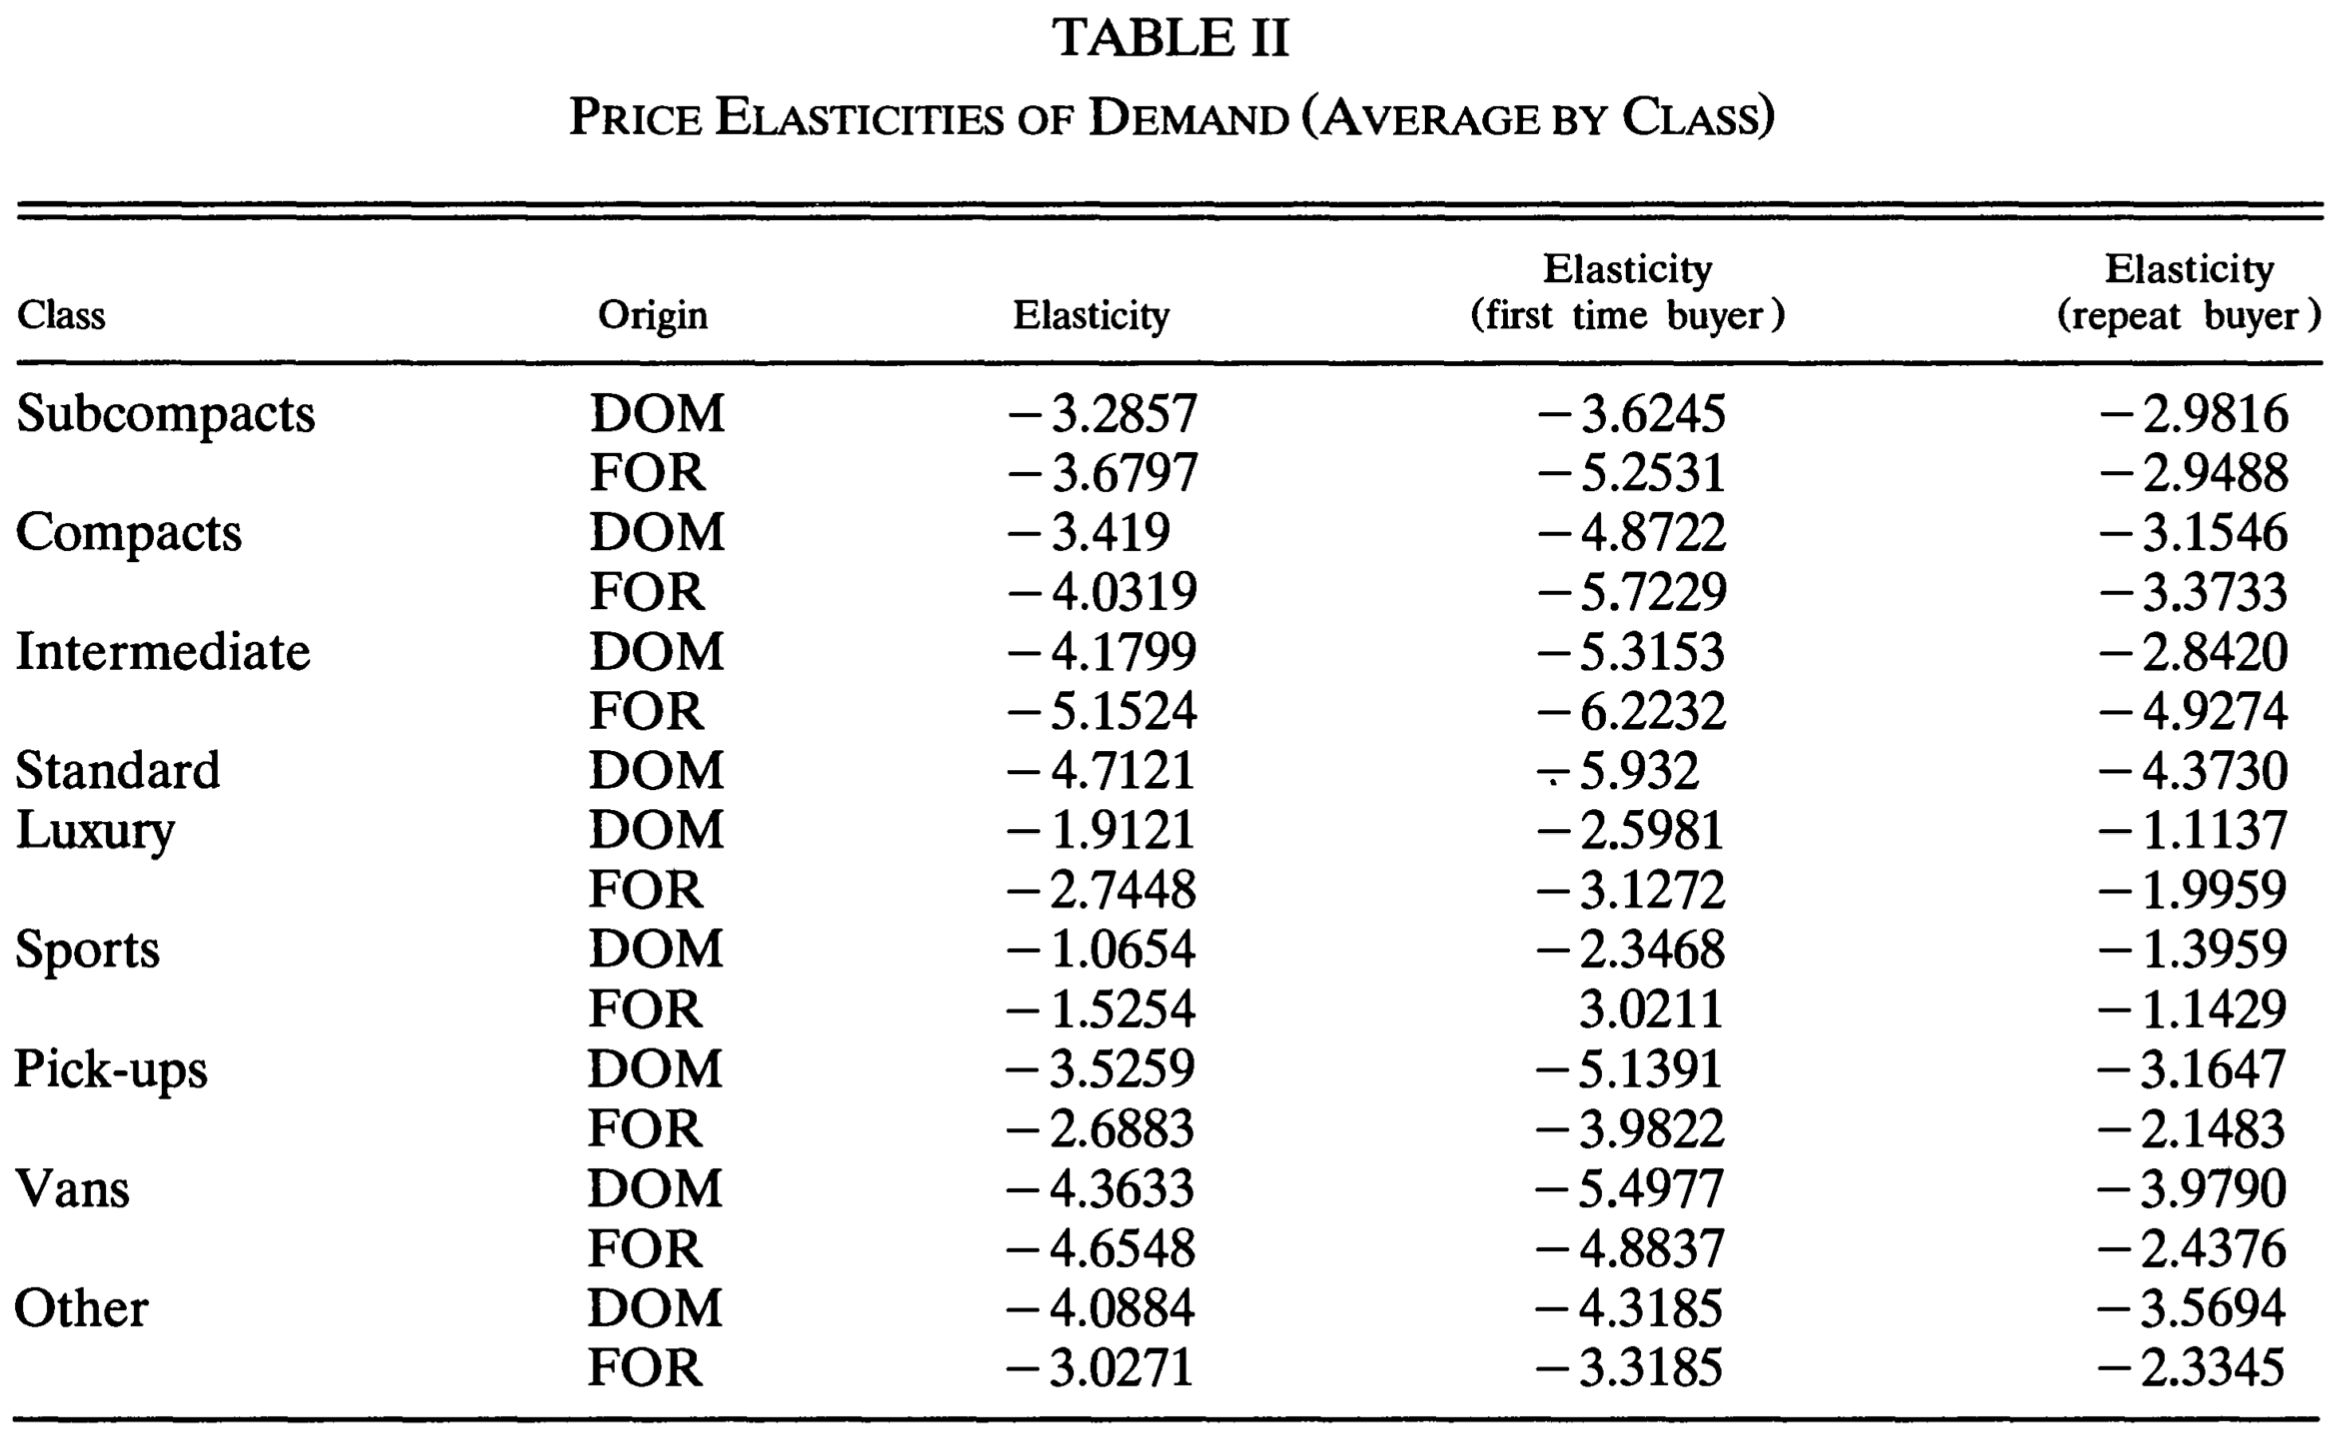
\includegraphics[scale=0.37]{table_2.png}
	\end{figure}
\end{frame}
%------------------------------------------------
\begin{frame}{Price Elasticities of Demand}
	\begin{figure}[h]
		\centering
		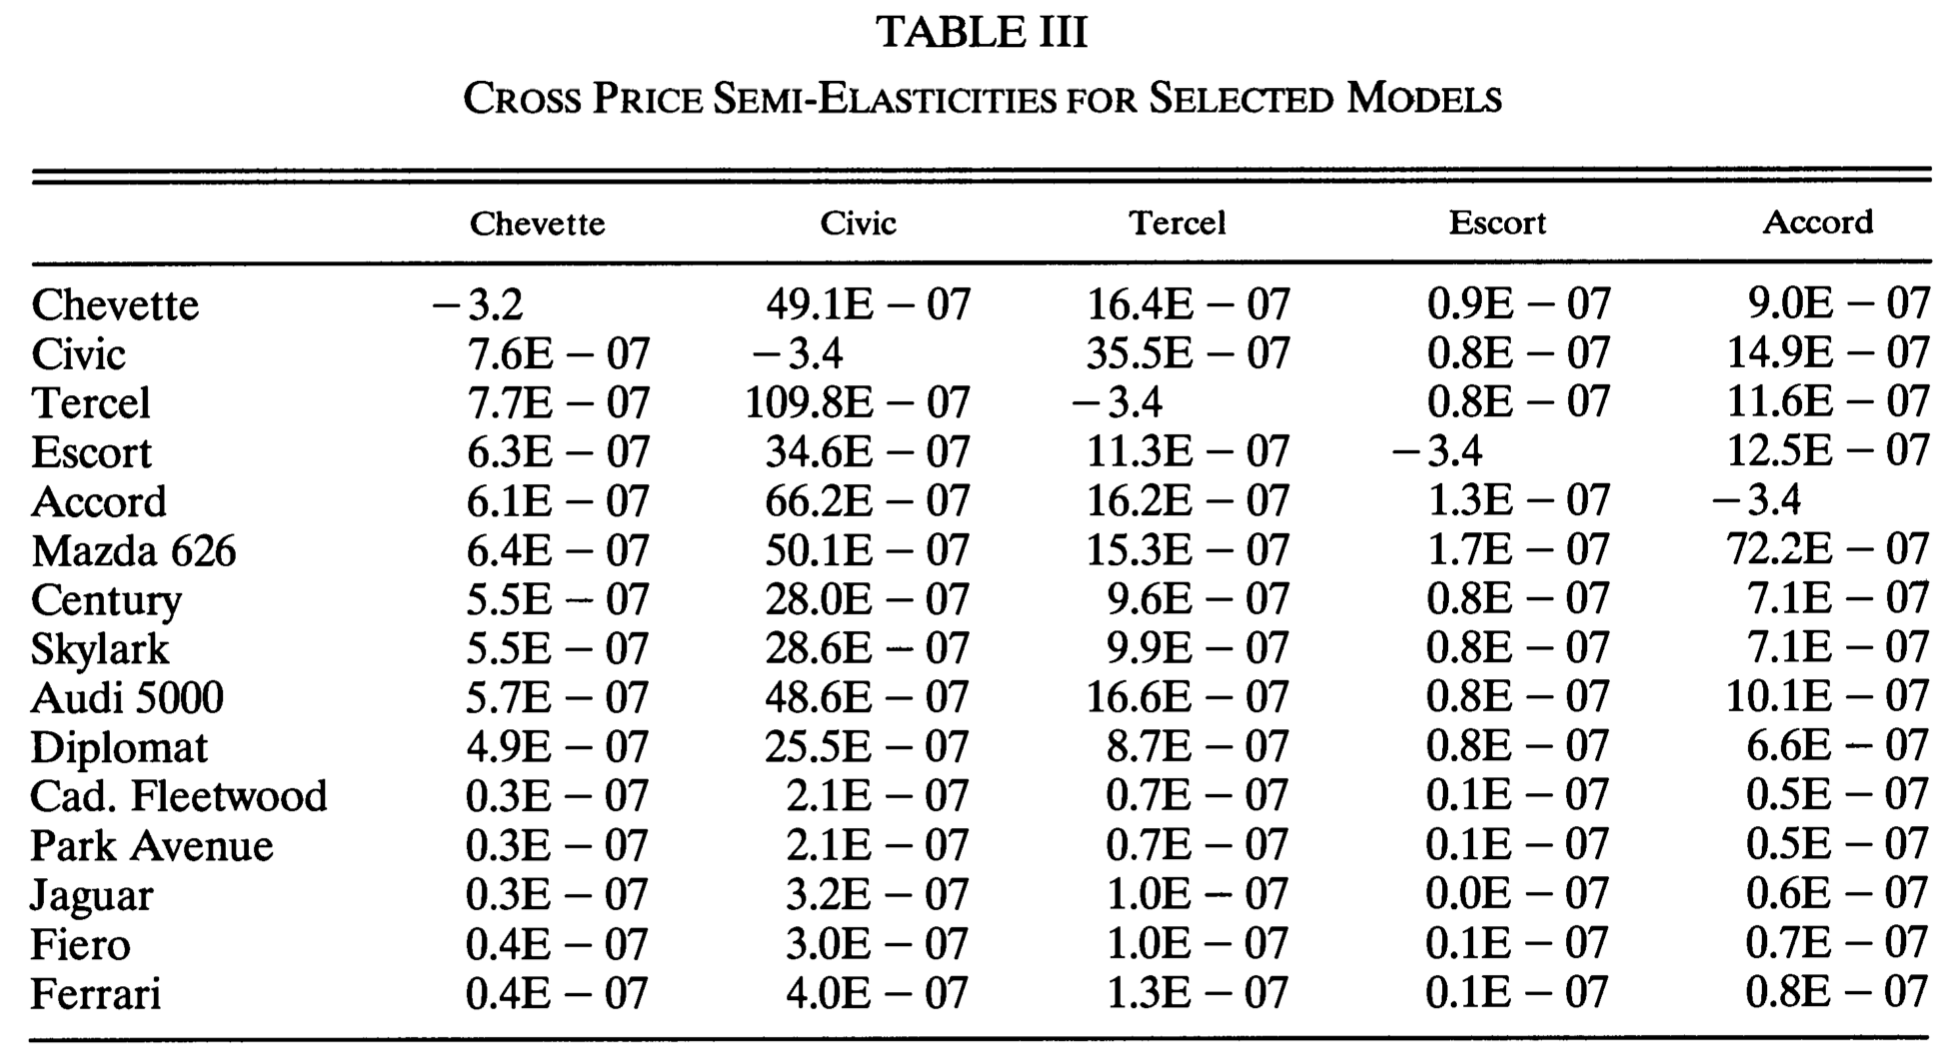
\includegraphics[scale=0.45]{table_3.png}
	\end{figure}
\end{frame}
%------------------------------------------------
\begin{frame}{Marginal Costs and Markups}
	The first order conditions for profit maximization can be solved for the marginal cost of each product. Then the markup for a specific model can be calculated as
	\begin{equation}
		\mbox{Markup}=\frac{\mbox{Wholesale Price}-\mbox{Marginal Cost}}{\mbox{Wholesale Price}}.
	\end{equation}

	According to my calculations, markups are on average 38\% while previous studies of the industry estimated them to be around 15\%. Why?
	\begin{itemize}
		\item Treating a fraction of the payroll as fixed cost would bring marginal costs closer to our estimates.
		\item Our cost estimates refer to short run marginal cost which in periods of capacity underutilization can be substantially lower than the average production cost.
		\item Bresnahan and Reiss (1985) find that the ratio of dealer to manufacturer markups is 0.71; 0.5 is not rejected. According to Consumer Reports, dealer markups are between 15 and 25\%, which implies manufacturer margins are between 22 and 50\%.
	\end{itemize}
\end{frame}
%------------------------------------------------
\begin{frame}{Marginal Costs and Markups}
	\begin{figure}[h]
		\centering
		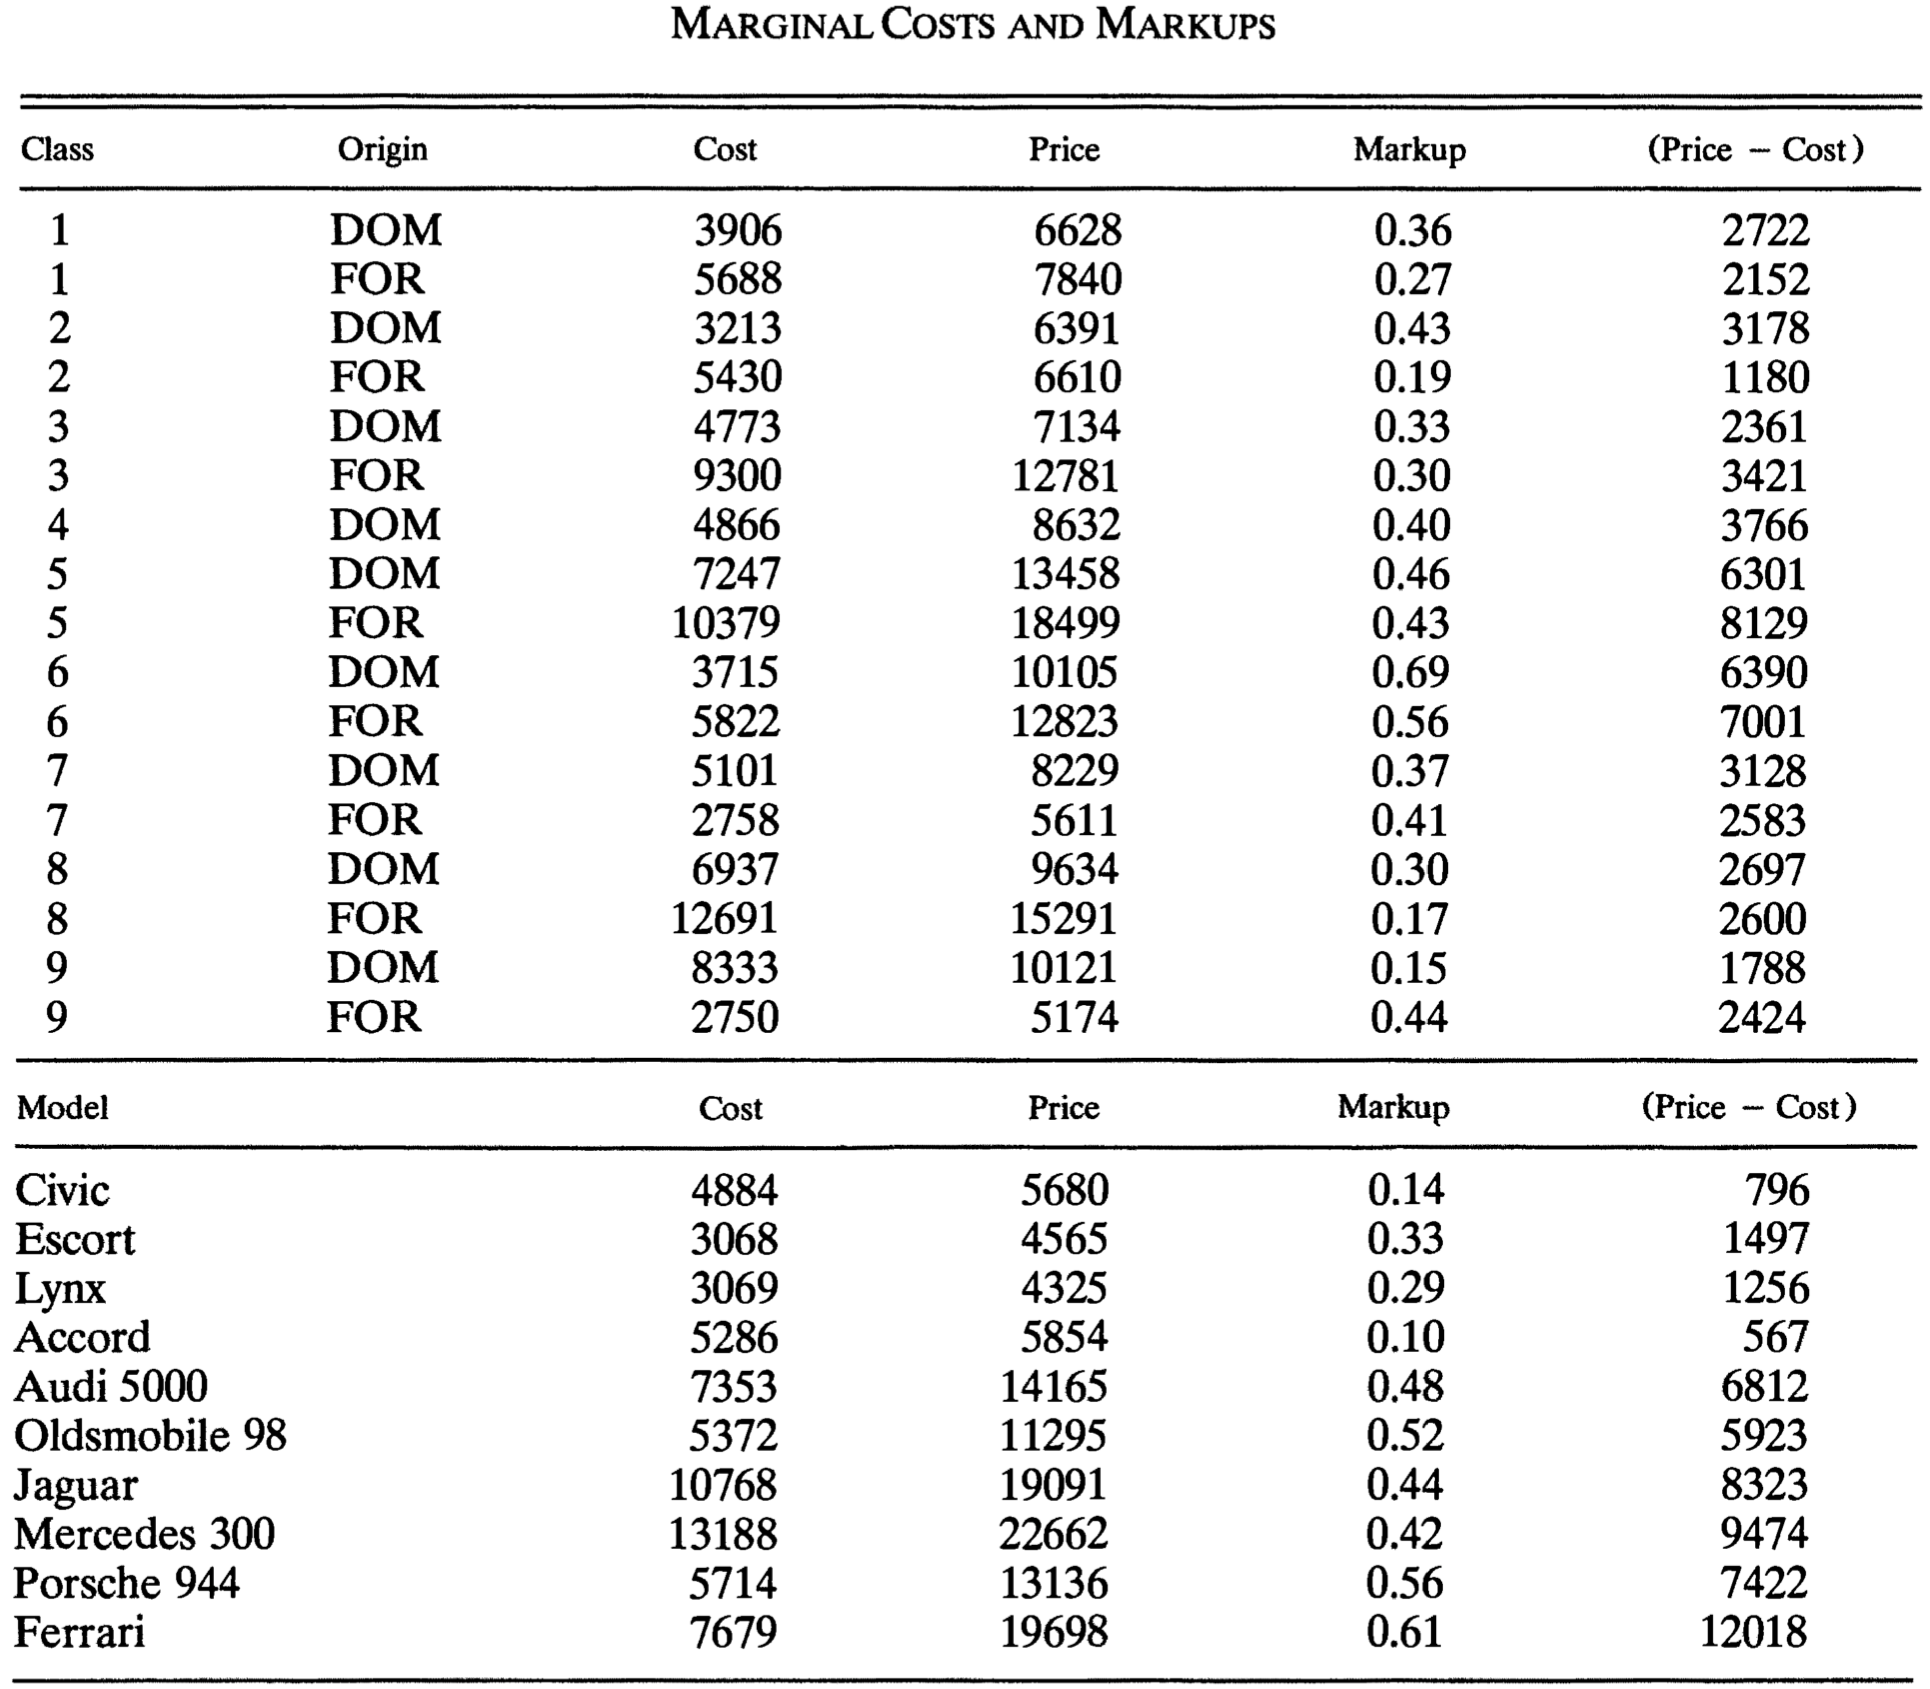
\includegraphics[scale=0.35]{table_4(2).png}
	\end{figure}
\end{frame}
%------------------------------------------------
\begin{frame}{Cost Parameters}
	The parameters of the cost function are estimated by regressing the estimated marginal costs of specific automobile models on vehicle characteristics and year dummies. An implicit assumption is that the marginal cost of an additional unit of a vehicle characteristic, expressed in the producer's local currency, is constant over the period 1983-87.
	\begin{itemize}
		\item The variables "QUOT1-QUOT5" are dummies specific to Japanese passenger cars that have been interacted with year dummies, which can be treated as year dummies, specific to the firms that produce cars subject to quotas.
		\item The estimated coefficients suggest that the quantity constraint was binding throughout the 1983-87 period, and had the strongest effects in the first three years.
	\end{itemize}
\end{frame}
%------------------------------------------------
\begin{frame}{Cost Parameters}
	\begin{columns}
		\column{0.33\textwidth}
		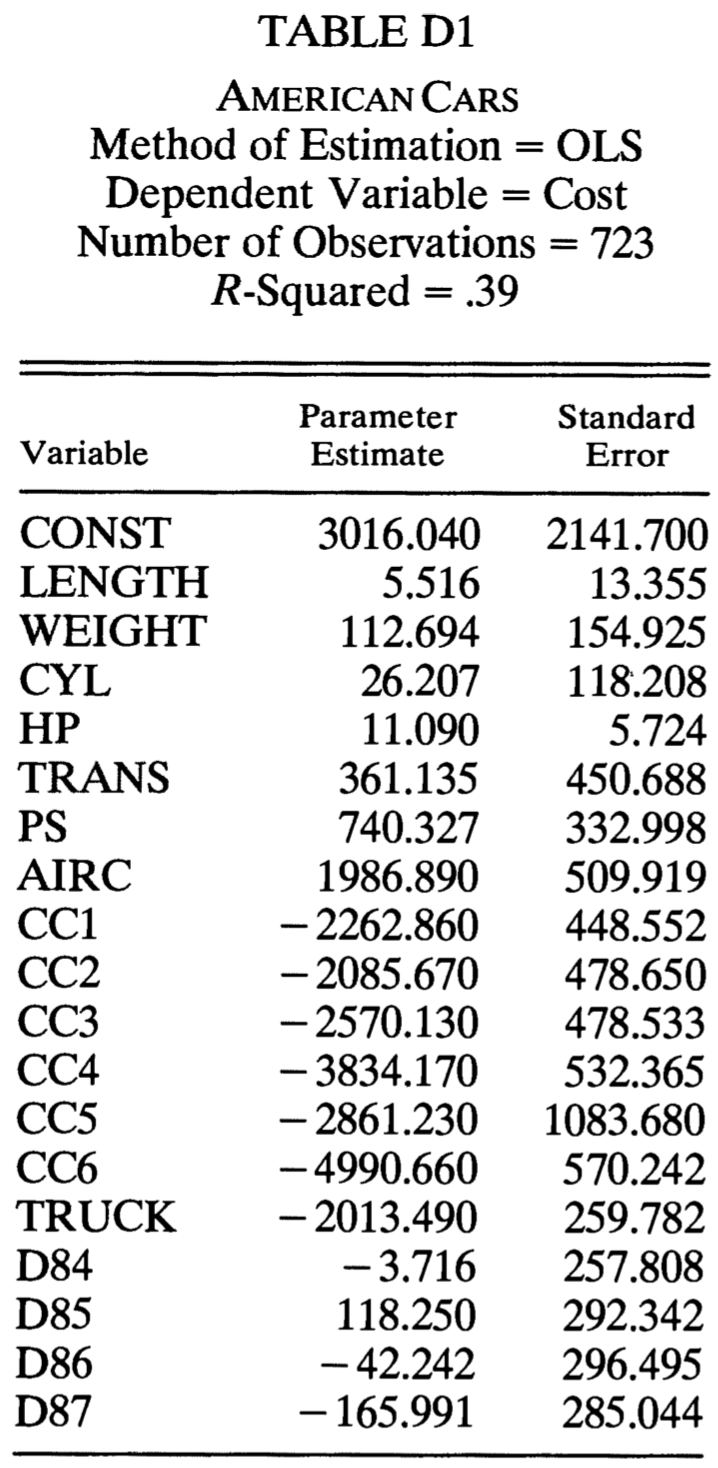
\includegraphics[width=3.5cm]{table_d1.png}
		\column{0.33\textwidth}
		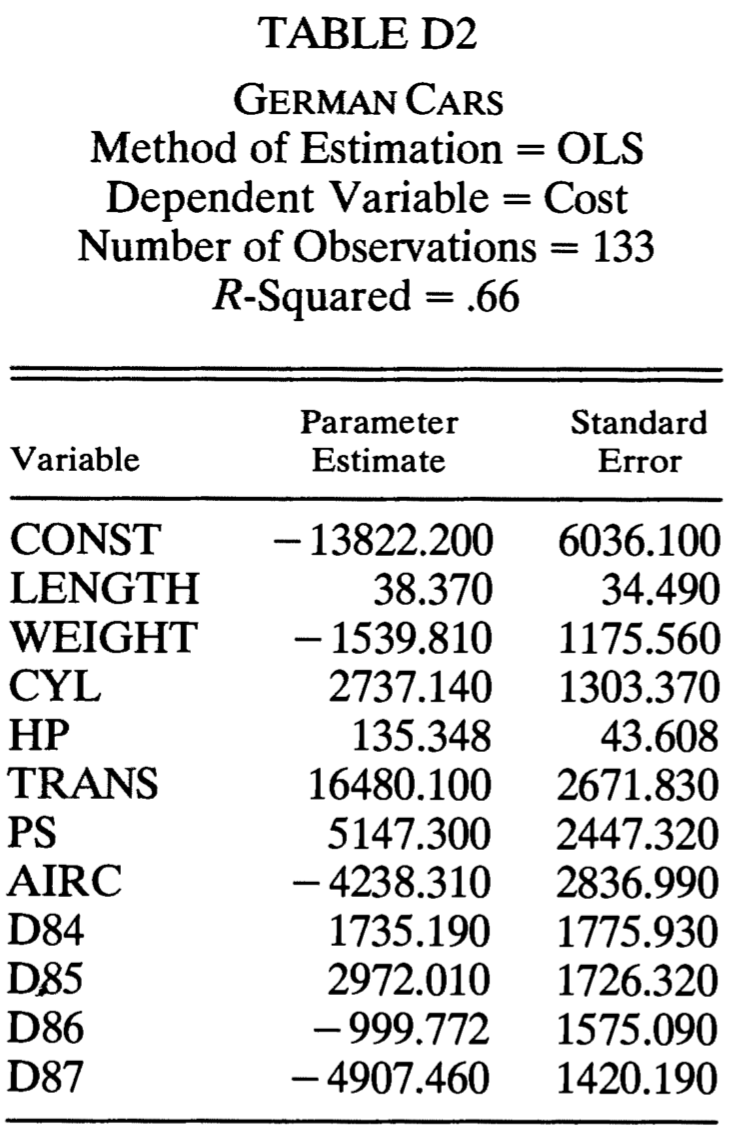
\includegraphics[width=3.7cm]{table_d2.png}
		\column{0.33\textwidth}
		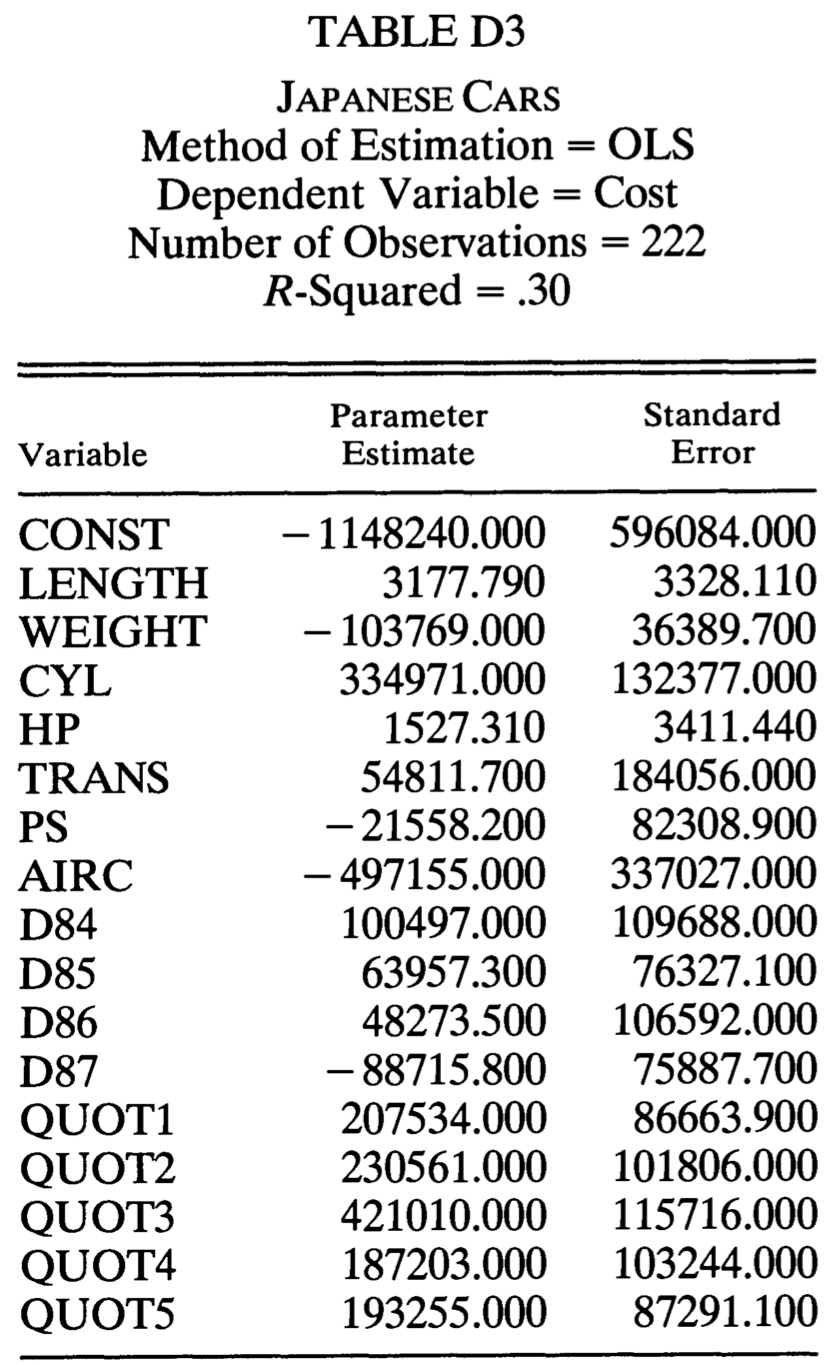
\includegraphics[width=3.5cm]{table_d3.png}
	\end{columns}
\end{frame}
%------------------------------------------------
\section{Model Applications}
\begin{frame}[shrink]
	\transfade %fade in and fade out
	\tableofcontents[sectionstyle=show/shaded,subsectionstyle=show/shaded/hide]
	\addtocounter{framenumber}{-1}
\end{frame}
%------------------------------------------------
\begin{frame}{Quotas}

	\textbf{background}:
	
	\begin{itemize}
	   \item  For the April, 1981-March, 1984 period, Japanese sales to the United States were subject to a limit of 1,832,500 cars per year.
	   \item  In April, 1984 the constraint was raised to 2,016,000 units.
	   \item The following year the Japanese government volunteered to limit Japanese auto sales in the U.S. market to 2.5 million annually, and has continued this policy ever since.
	\end{itemize}

	\textbf{Research Question}:
	\begin{enumerate}
	   \item Were the quota constraints binding during the 1983-87 period?
	   \item How did the export restraint affect the equilibrium outcome in the automobile industry? In particular what were the effects on sales and market shares, on prices, and on the quality mix?
	   \item How does the quota constraint compare to an equivalent tariff?
   \end{enumerate}
   
\end{frame}	


\begin{frame}{Quotas}{Were the quota constraints binding}

   Comparing the import shares with and without the quota constraint and examining the value of the Lagrange multiplier(components of the deterministic part of the marginal cost) in each year can provide insights as to the extent to which the export constraint was binding.

   \begin{figure}[h]
	   \centering          			
	   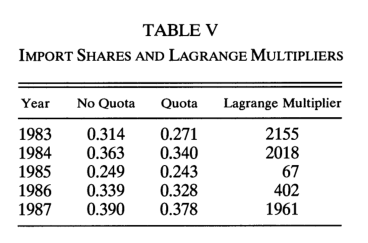
\includegraphics[scale=1.4]{table5.png}
	   \end{figure} 
\end{frame}	



\begin{frame}{Quotas}{The Quota Effects}

  Solve the model under two different assumptions, quotas vs. free trade, and compare the outcomes.

   \begin{itemize}
	   \item  Effects on Sales and Market Shares
	  
	 \end{itemize}

   \begin{figure}[h]
	   \centering          			
	   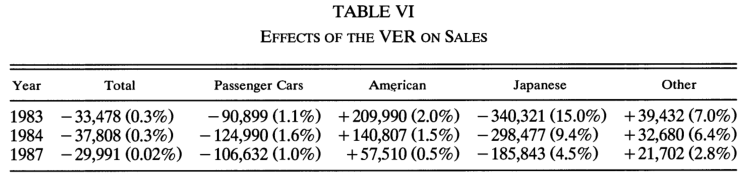
\includegraphics[scale=1.0]{table6.png}
	   \end{figure} 

	   \begin{itemize}
	   \item  Price Effects
   \end{itemize}

	In general, quotas raise prices:
	   
   The price increase is most pronounced in Japanese passenger cars subject to quotas, which experience an average increase of 14\% each year during 1983-84.63 The prices of domestic vehicles and other imports also rise, but less (0.5-0.9\% per year)
\end{frame}	



\begin{frame}{Quotas}{The Quota Effects}

   \begin{itemize}
	   \item Effects on Quality
	  
	 \end{itemize}

	 \textbf{quality upgrading}:
	 a movement towards market segments that include more expensive car

   \begin{figure}[h]
	   \centering          			
	   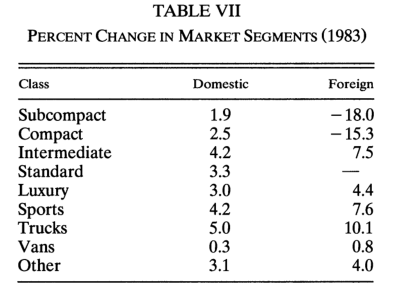
\includegraphics[scale=0.7]{table7.png}
	   \end{figure} 

	   \begin{itemize}
	   \item The decrease in Japanese subcompact sales is larger than the
	   corresponding decrease of compact sales.
	   \item The share of higher priced intermediate, standard, and luxury automobiles in both the American and the foreign production rises.
   \end{itemize}

	   The overall "quality" of automobile sales increases.
\end{frame}	



\begin{frame}{Quotas}{Comparison to an Equivalent Tariff}

   \begin{itemize}
	   \item Tariff on Japanese Imports
	   \item General Tariff on Imports
	  
	 \end{itemize}

   \begin{figure}[h]
	   \centering          			
	   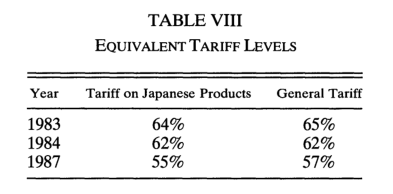
\includegraphics[scale=1.2]{table8.png}
	   \end{figure} 

   Because the different pass-through patterns between Japanese and other, primarily German, imports.
\end{frame}	


\begin{frame}{Quotas}{Summary}
	\begin{itemize}
		\item In summary, the impact of the VER on domestic production and therefore domestic employment was rather limited. In contrast, the price effects of the quota constraint were significant:
		\item The prices of new automobiles increased slightly, reducing purchases of new cars, while the relative prices of higher priced cars decreased, inducing a shift towards higher quality imports.
	\end{itemize}
\end{frame}	


\begin{frame}{Exchange Rate Pass-Through in the Automobile Industry}{Sylized facts}
	During the 1980's, the dollar experienced dramatic swings which were not reflected in the import prices of foreign automobiles.

   \begin{itemize}
	   \item Q1:What are the implications of the model with respect to exchange rate pass-through?
	   
	   \item Q2: if incorporating quota restrictions and quality change, can the model reproduce the price patterns observed during
	   1983-87?
	\end{itemize}

\end{frame}	


\begin{frame}{Exchange Rate Pass-Through in the Automobile Industry}

   Q1:What are the implications of the 	   model with respect to exchange rate pass-through?

	   \begin{figure}[h]
		   \centering          			
		   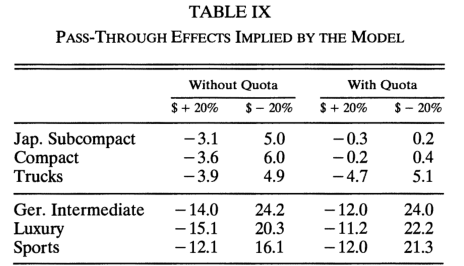
\includegraphics[scale=0.8]{table9.png}
		   \end{figure} 

   \begin{enumerate}
	   \item Exchange rate pass-through on import prices is asymmetric %贬值比升值影响更大
	   \item The pass-through coefficient for Japanese cars is smaller than German's.
	   \item In the presence of a quota Japanese import prices are insensitive to exchange rate movements.
	  
	 \end{enumerate}

	 \textbf{Explanation}:The model suggests that price elasticities for Japanese and German cars differ

\end{frame}	

% \begin{frame}
%     \frametitle{6.MODEL APPLIATIONS}
%     \textbf{6.2 Exchange Rate Pass-Through in the Automobile Industry}

%     Q1:What are the implications of the
%         model with respect to exchange rate pass-through?

%     \textbf{Explanation}:

%         The model suggests that price elasticities for Japanese and German cars differ.
%     \end{frame}	

\begin{frame}{Exchange Rate Pass-Through in the Automobile Industry}

   Next, apply the model to 1983-87. Price movements across years are the result of three component:

   \begin{enumerate}
	\item quota restriction
	\item exchange rate changes
	\item quality change of vehicle makes

   \end{enumerate}

   Compute the equilibrium in each period holding two of the three components
   constant


\end{frame}


\begin{frame}{Exchange Rate Pass-Through in the Automobile Industry}

   \begin{figure}
	   \begin{minipage}[t]{0.35\linewidth}
		   \centering
		   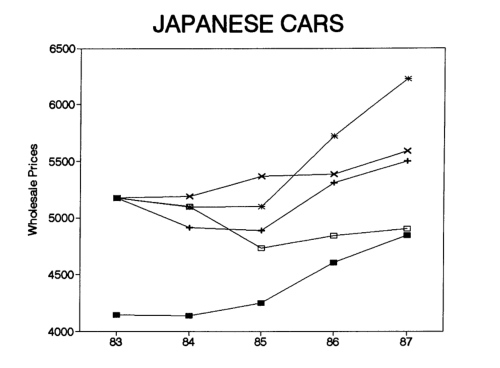
\includegraphics[height=3.5cm,width=6cm]{t11.png}
		   \end{minipage}%
		   \hfill
		   \begin{minipage}[t]{0.5\linewidth}
		   \centering
		   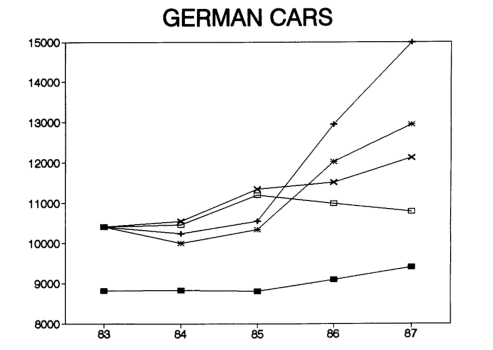
\includegraphics[height=3.5cm,width=6cm]{t12.png}
		   \end{minipage}

	   \end{figure}
	   \begin{figure}[h]
		   \centering          			
		   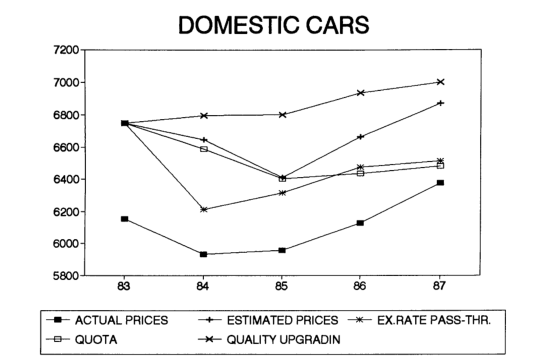
\includegraphics[scale=0.8]{t111.png}
		   \end{figure} 
\end{frame}  


\begin{frame}{Exchange Rate Pass-Through in the Automobile Industry}{Conclusions}
   \begin{enumerate}
	   \item  Exchange rate pass-through cannot be
	   analyzed without considering the impact of trade restrictions and quality change
	   on import prices

	   \item the static model is useful in predicting actual prices
	   when the dollar appreciates, but not as useful when it depreciate.

	   Because the model ignores the influence of demand
	   dynamics on profit maximization.

   \end{enumerate}

\end{frame}

%------------------------------------------------
\begin{frame}
\Huge{\centerline{\textit{The End}}}
\end{frame}
%----------------------------------------------------------------------------------------


\end{document} 